\documentclass{article}
\usepackage[utf8]{inputenc}
\usepackage{graphicx}
\usepackage{subcaption}
\usepackage{titling}
\usepackage{booktabs}
\usepackage{amsmath}
\usepackage{lipsum}
\usepackage{cmbright}
\usepackage[T1]{fontenc}
\usepackage{tabularx} 
\usepackage{multirow}
\usepackage{bm}
\usepackage[colorlinks=true, linkcolor=red, urlcolor=blue, citecolor=red]{hyperref}
\usepackage{geometry}
\geometry{
  a4paper,
  total={170mm,257mm},
  left=15mm,
  top=15mm,
}

\title{Seminar: Statistics for Data Science: Group C \\ Personal Agency vs.\ Environmental Determinism in Academic Success}
\author{Dmytro Tupkalenko (89252101), Natalia Tashkova (89252098), Yllk\"{e} Jashari (89252111) \\ University of Primorska, FAMNIT}
\date{Date of presentation: 07.05.2026}




\begin{document}

\maketitle




\newpage
\section{Introduction and Research Question}
\label{sec:introduction}

This study investigates the relative contribution of student-driven behavioral choices versus structural and environmental constraints in academic success. The guiding research question is: \textit{To what extent do student-driven behavioral choices are associated with academic success in Portuguese and Mathematics, compared to structural and environmental constraints?} All of the analysis is based on multiple linear regression, which is operationalized in two parts. First, a descriptive analysis where we look at the identified associations, compare them across the constructed profiles (structural and structural + behavioral) and subjects. Second, a predictive analysis where we compare the models fitted on only structural and on full profiles in terms of their predictive and explanatory power. 


\paragraph{Note}

This report follows the timeline of the analysis. As a result, some concepts are presented as they were understood at each stage, even though they were later refined or revised in subsequent sections.


\paragraph{Sample Description}

The sample consists of students aged between 15 and 22 who are enrolled in Mathematics and Portuguese language courses at two secondary schools in Portugal: Gabriel Pereira and Mousinho da Silveira. The data comes from two datasets, one per subject, merged on a shared set of students, yielding 370 students.


\paragraph{Included Variables}

Based on the research question, all variables were assigned to one of three groups. \textit{Structural} predictors capture fixed background constraints outside the student's control such as family composition, parental education, and access to resources. \textit{Behavioral} predictors capture choices the student actively makes, such as study time, going out, and alcohol consumption. \textit{General} demographic variables are included as controls in both models. The measure of academic success in this study is defined as final grade in the subject. Below is table summarizing this:


\begin{table}[h!]
\centering
\footnotesize         
\begin{tabularx}{\textwidth}{llXp{4.5cm}X}
\toprule
\textbf{Group} & \textbf{Variable} & \textbf{Description} & \textbf{Type} & \textbf{Motivation} \\
\midrule
\multicolumn{5}{l}{\textit{General}} \\
\midrule
& \texttt{school} & Student's school         & Binary (GP / MS)    & Environmental control. \\
& \texttt{sex}    & Student's sex            & Binary (F / M)      & Demographic control. \\
& \texttt{age}    & Student's age            & Numeric (15--22)    & Demographic control. \\
\midrule
\multicolumn{5}{l}{\textit{Structural / Environmental --- something that a student cannot control}} \\
\midrule
& \texttt{address}      & Home address type            & Binary (Urban / Rural)                                        & Access to urban resources. \\
& \texttt{famsize}      & Family size                  & Binary ($\leq$3 / $>$3)                                       & Home study environment. \\
& \texttt{Pstatus}      & Parent's cohabitation status & Binary (Together / Apart)                                     & Home-life stability. \\
& \texttt{Medu}$^{**}$  & Mother's education           & Ordinal (none / primary / 5th--9th / secondary / higher)      & Socioeconomic and cultural capital. \\
& \texttt{Fedu}$^{**}$  & Father's education           & Ordinal (none / primary / 5th--9th / secondary / higher)      & Complements \texttt{Medu}. \\
& \texttt{traveltime}   & Home to school travel time   & Ordinal ($<$15 min / 15--30 min / 30 min--1 h / $>$1 h)       & Amount of "dead time" --- limits available study time. \\
& \texttt{internet}     & Internet access at home      & Binary (yes / no)                                             & Access to online study materials. \\
& \texttt{health}       & Current health status        & Ordinal (1=very bad ... 5=very good)                          & Baseline capacity to perform. \\
\midrule
\multicolumn{5}{l}{\textit{Behavioural --- something that a student can control}} \\
\midrule
& \texttt{studytime}    & Weekly study time             & Ordinal ($<$2 h / 2--5 h / 5--10 h / $>$10 h)                & Most direct proxy for personal effort. \\
& \texttt{goout}        & Going out with friends        & ordinal (1=very low ... 5=very high)                         & Time allocation and social priorities. \\
& \texttt{activities}.  & Extra-curricular activities   & Binary (yes / no)                                            & Proactive non-academic engagement. \\
& \texttt{romantic}     & In a romantic relationship    & Binary (yes / no)                                            & Competing demands on time and energy. \\
& \texttt{Walc}$^{*}$   & Weekend alcohol consumption   & Ordinal (1=very low ... 5=very high)                         & Weekend lifestyle choices. \\
& \texttt{Dalc}$^{*}$   & Workday alcohol consumption.  & Ordinal (1=very low ... 5=very high)                         & Daily cognitive readiness. \\
\midrule
\multicolumn{5}{l}{\textit{Outcome}} \\
\midrule
& \texttt{G3} & Final grade & Numeric (0--20) & Academic success. \\
\bottomrule
\end{tabularx}
\label{tab:variables}
\end{table}

\noindent
Note that variables marked with * and ** respectively are hypothesized to be strongly associated, but are still included in the initial set with the possibility to be ruled out after Initial Data Analysis.


\paragraph{Excluded Variables}

Remaining variables available in the dataset were excluded to maintain focus on the research question. Past academic performance metrics (\texttt{G1}, \texttt{G2}, and past \texttt{failures}) were removed; because including these would overwhelm model accuracy which we want to compare in isolated manner. Family occupation variables (\texttt{Mjob}, \texttt{Fjob}, and \texttt{guardian}) were excluded because \texttt{Medu} and \texttt{Fedu} were considered sufficient proxies for socioeconomic status; although \texttt{Mjob} and \texttt{Fjob} could be useful additions, they are recorded as nominal job-type labels (`teacher'', `health'', `services'', `at\_home'', ``other'') that do not map onto any measurable metric such as family capital. \texttt{schoolsup}, \texttt{famsup}, \texttt{paid}, \texttt{nursery}, \texttt{higher}, \texttt{freetime}, and \texttt{famrel} were omitted because they could not be strictly classified as either behavioral or structural --- for example, attending paid lessons may reflect parental initiative as much as the student's own choice (e.g. the situation in which student would attend them, but family budget does not allow it).


\paragraph{Statistical Approach}

To address both research questions, we fit \textbf{four multiple linear regression models in total} --- two for Mathematics and two for Portuguese. For each subject, a \textit{Structural Model} includes only the general controls and environmental constraints:
\[
  G3 = \beta_0
       + \sum_{j\,\in\,\text{General}} \beta_j X_j
       + \sum_{k\,\in\,\text{Structural}} \beta_k X_k
       + \epsilon,
\]
while the \textit{Full Model} extends it with the behavioural predictors:
\[
  G3 = \beta_0
       + \sum_{j\,\in\,\text{General}} \beta_j X_j
       + \sum_{k\,\in\,\text{Structural}} \beta_k X_k
       + \sum_{l\,\in\,\text{Behavioural}} \beta_l X_l
       + \epsilon.
\]

Models predictice power are evaluated using RMSE, MAE, and their leave-one-out cross-validated equivalents. Explanatory power is evaluated with AIC, $R^2$ and Adjusted $R^2$.

\vspace{0.5em}
Ordinal predictors are handled in two ways. \texttt{Medu}, \texttt{Fedu}, \texttt{studytime}, and \texttt{traveltime} are encoded as ordered factors with successive difference contrasts, because their categories represent qualitatively distinct thresholds with non-uniform spacing. The remaining ordinal variables --- \texttt{goout}, \texttt{Dalc}, \texttt{Walc}, and \texttt{health} --- are treated as numeric. These are symmetric 5-point Likert-style scales, and encoding each as a factor would consume an additional 4 degrees of freedom each that the sample cannot afford (discussed further).




\section{Initial Data Analysis}
\label{sec:ida}
In this section we report the findings from Initial Data Analysis (IDA), which included missing value analysis, univariate analysis, multivariate analysis and redundancy analysis.



\subsection{IDA Screening: Missing Values}

There were no NAs in this dataset. However there were some valid encodings that were special (0 in G3, None in Parent's education) --- so we investigated these ones. Below we summarize the numbers in the table:

\begin{table}[h!]
\centering
\small
\begin{tabular}{lc}
\toprule
\multicolumn{2}{l}{\textit{Zero / Baseline Value Counts}} \\
\multicolumn{2}{l}{\footnotesize \texttt{Medu} \& \texttt{Fedu}: parents with no education; \texttt{G3}: students scoring 0} \\
\midrule
\textbf{Variable} & \textbf{$n$} \\
\midrule
\texttt{Medu} = None  & 3  \\
\texttt{Fedu} = None  & 2  \\
\texttt{G3} = 0 (Mathematics)   & 35 \\
\texttt{G3} = 0 (Portuguese)    & 5  \\
\bottomrule
\end{tabular}
\label{tab:zero_counts}
\end{table}

The first observation we could make is that for Medu = None and Fedu = None looking at the records, we could not understand whether these really correspond to not having education or they encode something else. Given that the presence of both is very small in the sample, which would even if the encodings are truthful not produce meaningful results (we used incremental contrast factors for these variables) in the model, we decided to exclude these records --- which resulted in 365 observations.

\vspace{0.2em}
The second observation is for G3 being 0, there is no specification in student.txt so we were not sure what is the meaning. We supposed that this corresponds to dropouts from the course, which if true would largely inflate our models; because we wanted to focus on the difference in final grades not whether the student finishes the course. To check the assumption that this corresponds to dropouts, we summarized these cases below.


\begin{table}[h!]
\centering
\small
\begin{tabular}{llcccccccc}
\toprule
& & & \multicolumn{7}{c}{\textbf{Predictor Means}} \\
\cmidrule(lr){4-10}
\textbf{Subject} & \textbf{Group} & \textbf{$n$} & \textbf{Age} & \textbf{Studytime} & \textbf{Goout} & \textbf{Dalc} & \textbf{Walc} & \textbf{Medu} & \textbf{Fedu} \\
\midrule
\multirow{2}{*}{Mathematics} & $G3 = 0$ &  35 & 17.03 & 2.03 & 3.17 & 1.31 & 1.86 & 3.40 & 3.31 \\
                             & $G3 > 0$ & 335 & 16.53 & 2.04 & 3.11 & 1.50 & 2.34 & 3.84 & 3.58 \\
\midrule
\multirow{2}{*}{Portuguese}  & $G3 = 0$ &   5 & 18.20 & 1.20 & 3.00 & 2.40 & 3.20 & 3.40 & 2.80 \\
                             & $G3 > 0$ & 365 & 16.55 & 2.05 & 3.12 & 1.47 & 2.28 & 3.81 & 3.57 \\
\bottomrule
\end{tabular}
\label{tab:zero_means}
\end{table}

What we observed is that, first in the Mathematics dataset, we observed that 12  students with a final grade of zero (G3 = 0) also lack recorded grades for the second period (G2) (for sake of space the full table is not reported here, just the number). Second, among their observable characteristics there is nothing indicating that these are some special group of students --- there are differences especially among Portuguese students; but they are just other indicators that these students are dropouts (e.g. higher alcohol consumption --- which is the characteristic that, we think, is generally agreed to be associated with not finishing some duty -\> dropping out). So, this pattern suggests that these cases most likely correspond to students who dropped out. As we discussed before, keeping them would distort the analysis, so, we excluded these observations --- which resulted in 327 observations that we used in the model fitting.



\subsection{IDA Screening: Univariate Analysis}

\subsubsection*{Continuous Variables}

The continuous variables in the dataset are age and the two final-grade
outcomes --- they were summarized with histograms and table (only histogram is reported here for the sake of space):

\begin{figure}[h!]
    \centering
    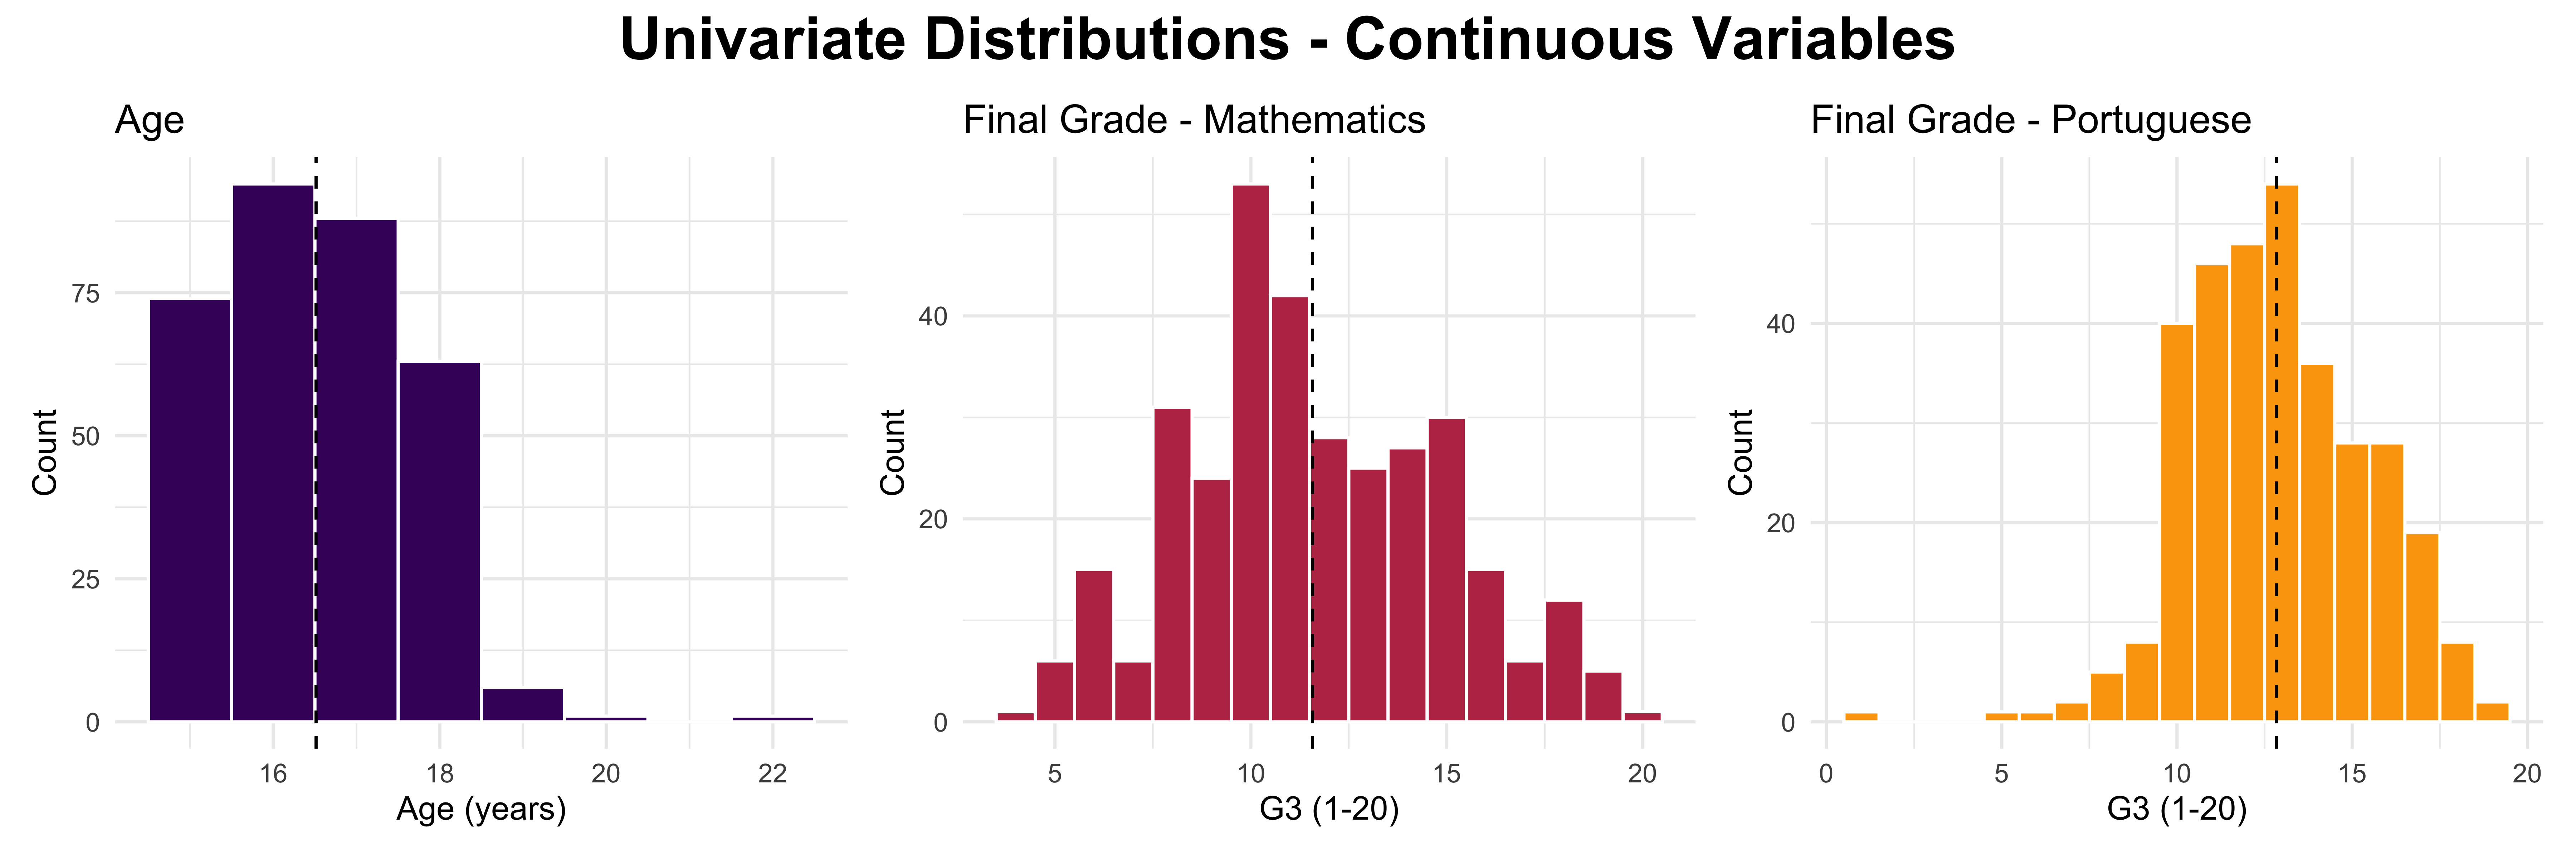
\includegraphics[width=\textwidth]{code_files/figure-html/ida_continuous_plots-1.png}
\end{figure}

\textbf{Age}, the distribution is concentrated in the 15--18 range, which together account for 97.5\% of the sample. The mean and median both sit at 16--17 years, as expected for secondary school students. The tail extends to age 22, with two isolated observations at ages 20 and 22 (one student each). The single 22-year-old is a potential anomaly, but in the documentation the range is (18--22), so we kept it.

\vspace{0.2em}
\textbf{G3 - Mathematics}, the distribution is roughly symmetric around the median and mean of 12, with grades ranging from 4 to 20. The most common grade is 10 (16.2\% of students), and the interquartile range spans 9--14, suggesting moderate spread.

\vspace{0.2em}
\textbf{G3 - Portuguese}, the distribution is more concentrated than Mathematics, with a mean and median both at 13 and a narrower IQR of 11--15. The distribution is approximately symmetric but with moderate left-skewness. There is one isolated observation at grade 1, which is notably lower than the next minimum of 5 --- this single case grabs attention, but given that we already excluded $G3 = 0$ as dropouts, we kept it.



\subsubsection*{Categorical Variables}

Note that the value of variables for Mathematics and Portuguese are the
same. So below we use data for Mathematics, but it is completely similar
for Portuguese. We summarize this with bar plots for ordinal and binary variables:

\begin{figure}[h!]
    \centering
    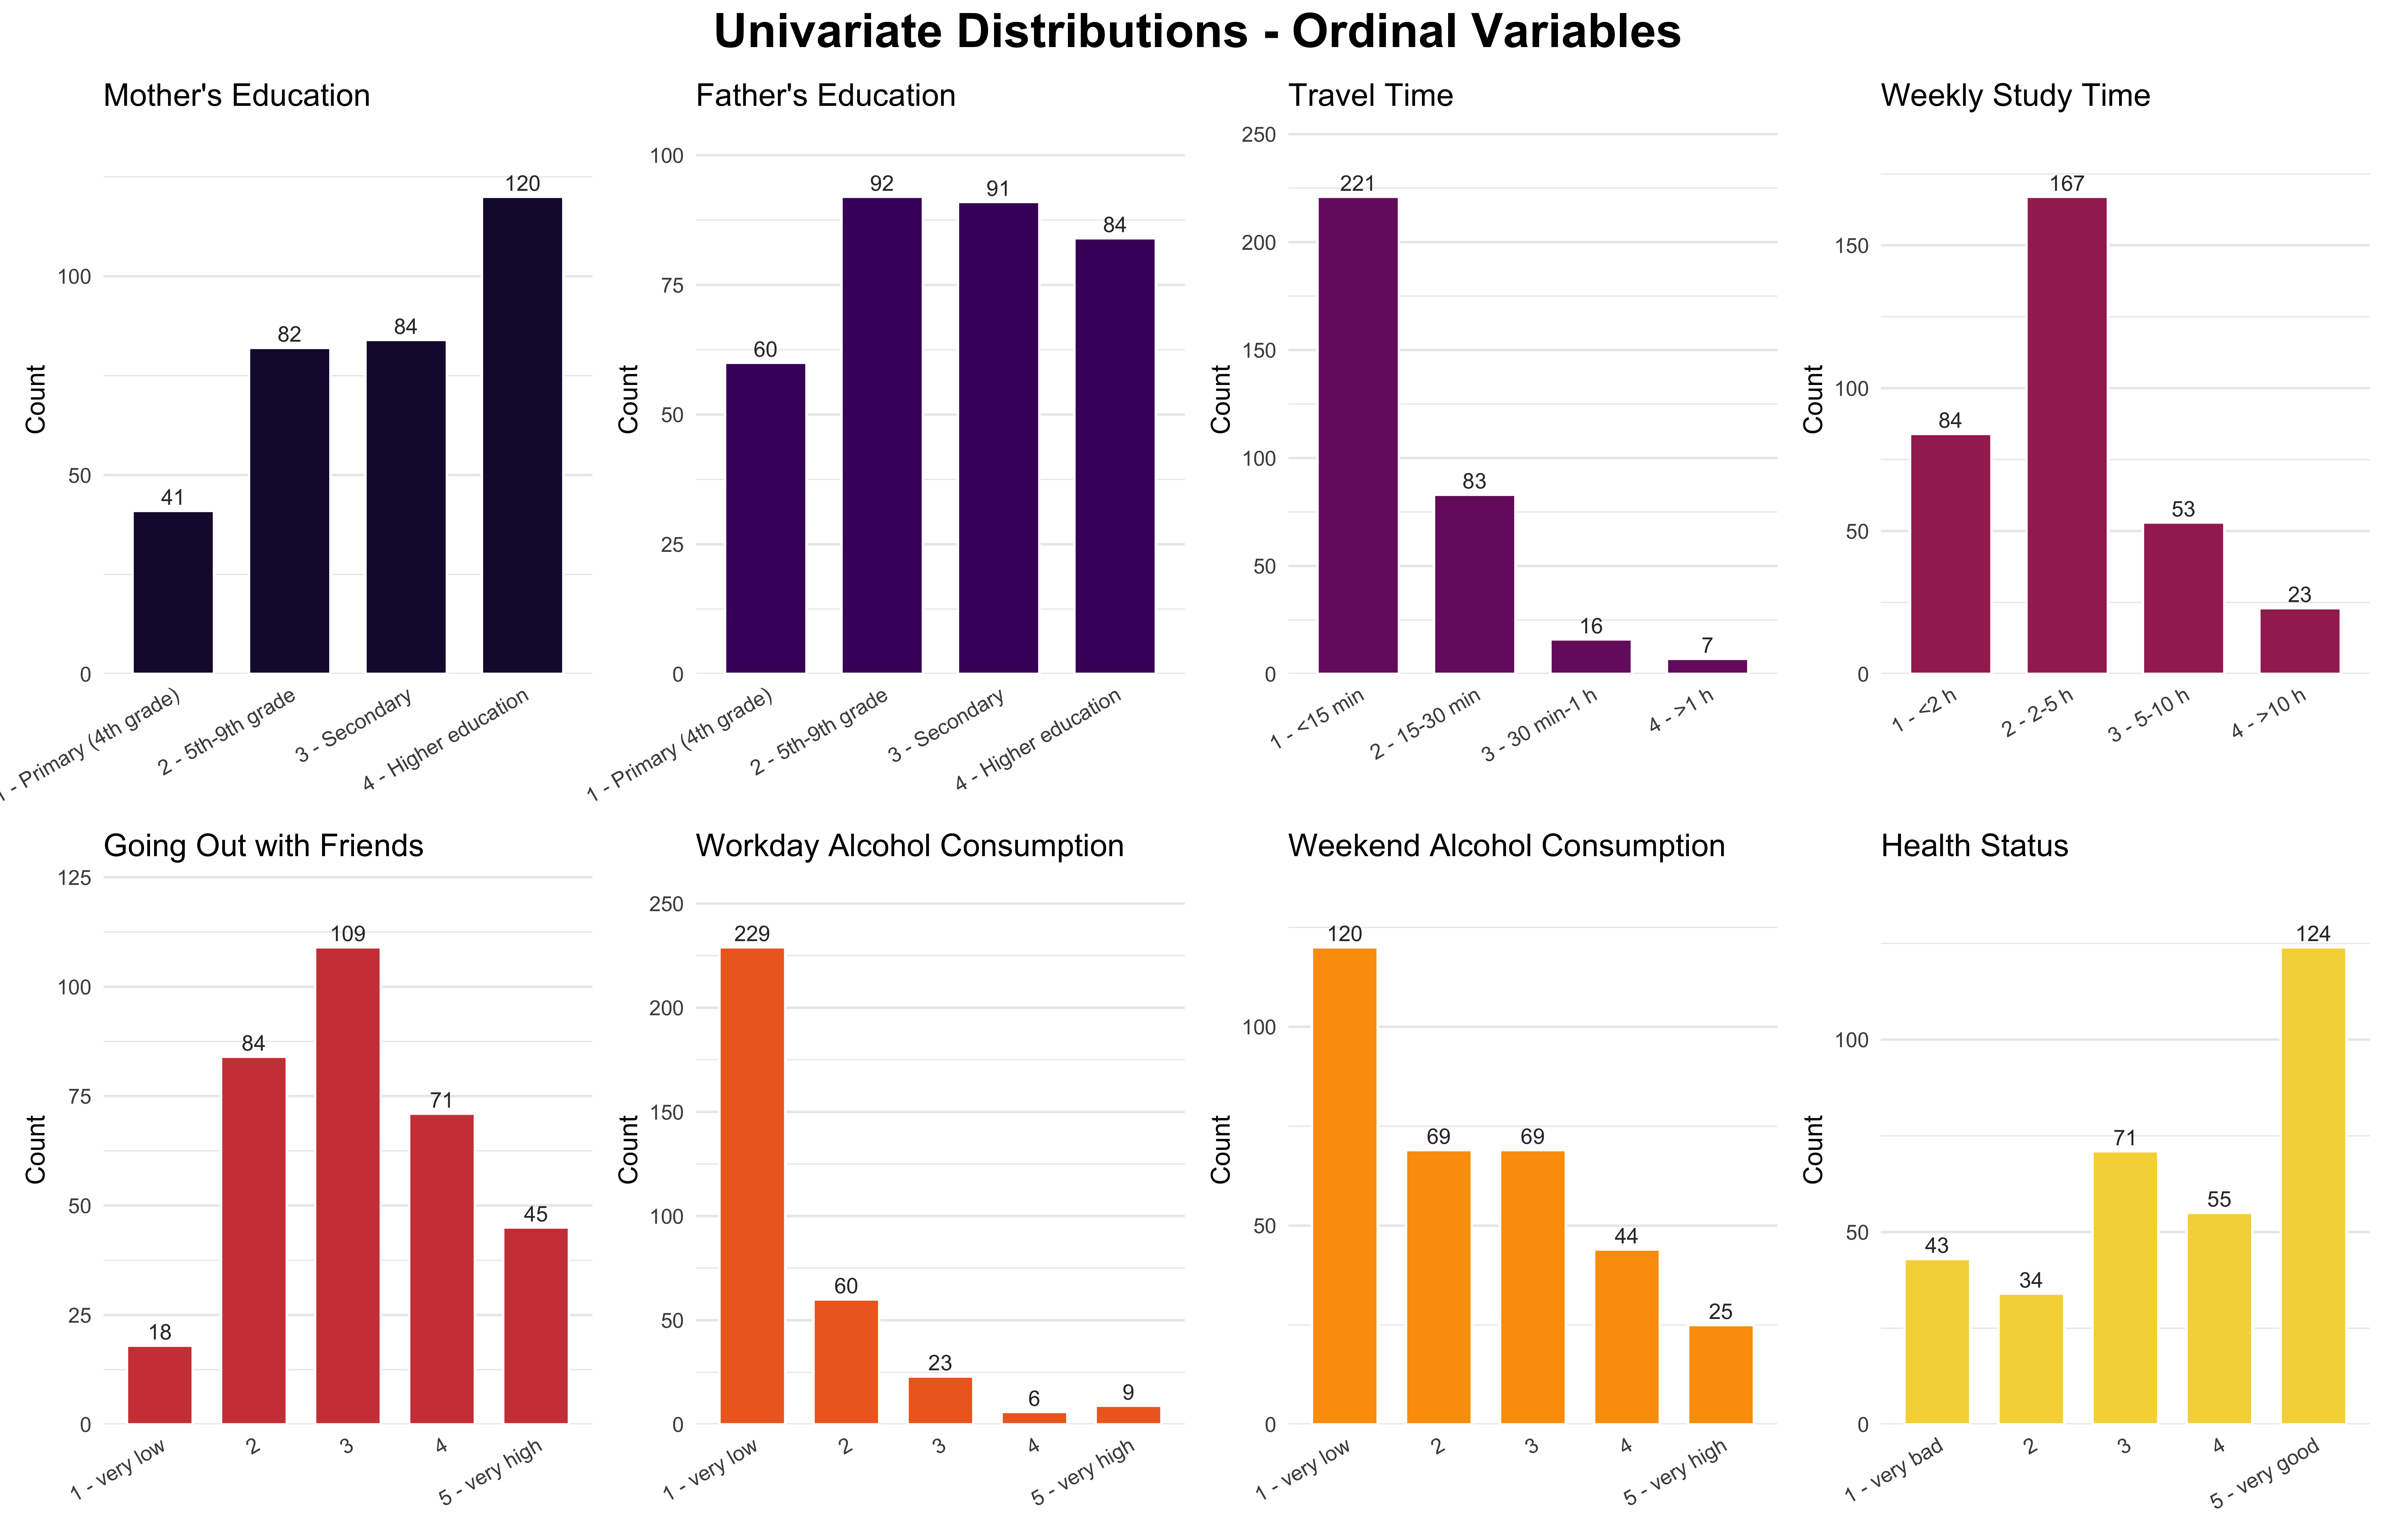
\includegraphics[width=\textwidth]{code_files/figure-html/ida_ordinal_plots-1.png}
\end{figure}

\newpage
\textbf{Medu and Fedu}: In the case of mother's education, the distribution is somewhat left-skewed, whereas the distribution for father's education is closer to uniform. This observation was kept until multivariate analysis, where one variable may be prioritized.

\vspace{0.2em}
\textbf{traveltime}: The distribution is right-skewed. The top two levels (16 and 7 observations) were merged into a single "\textgreater=30 min" category before model fitting, as small cell sizes in these strata would produce unstable coefficient estimates.

\vspace{0.2em}
\textbf{studytime}: The distribution is reasonably spread, with the majority studying 2–5 hours per week. The upper level (\textgreater10 hours) is the smallest group with only 23 students --- we thought of merging the two top categories, but in the end decided not to because we supposed that this is most likely one of the strongest predictors, and the strata size is small but not extremely.

\vspace{0.2em}
\textbf{goout}: The distribution is close to symmetric and centered on level 3. Level 1 ("very low") has only 18 students, which is notably sparse relative to the remaining levels, but since we code it as numeric, this should not play a significant role.

\vspace{0.2em}
\textbf{Dalc and Walc}: These distributions differ notably; Dalc is heavily concentrated at "very low" (approximately 70.0\%), with very sparse counts at levels 4 and 5. Walc is more spread across all levels, with counts for levels 4 and 5 still somewhat underrepresented but sufficient to retain as separate levels. Given their expected collinearity, the decision on retaining or excluding either variable was left until multivariate analysis.

\vspace{0.2em}
\textbf{health}: The distribution is left-skewed. All five levels have reasonable counts.

\vspace{-0.2em}
\begin{figure}[h!]
    \centering
    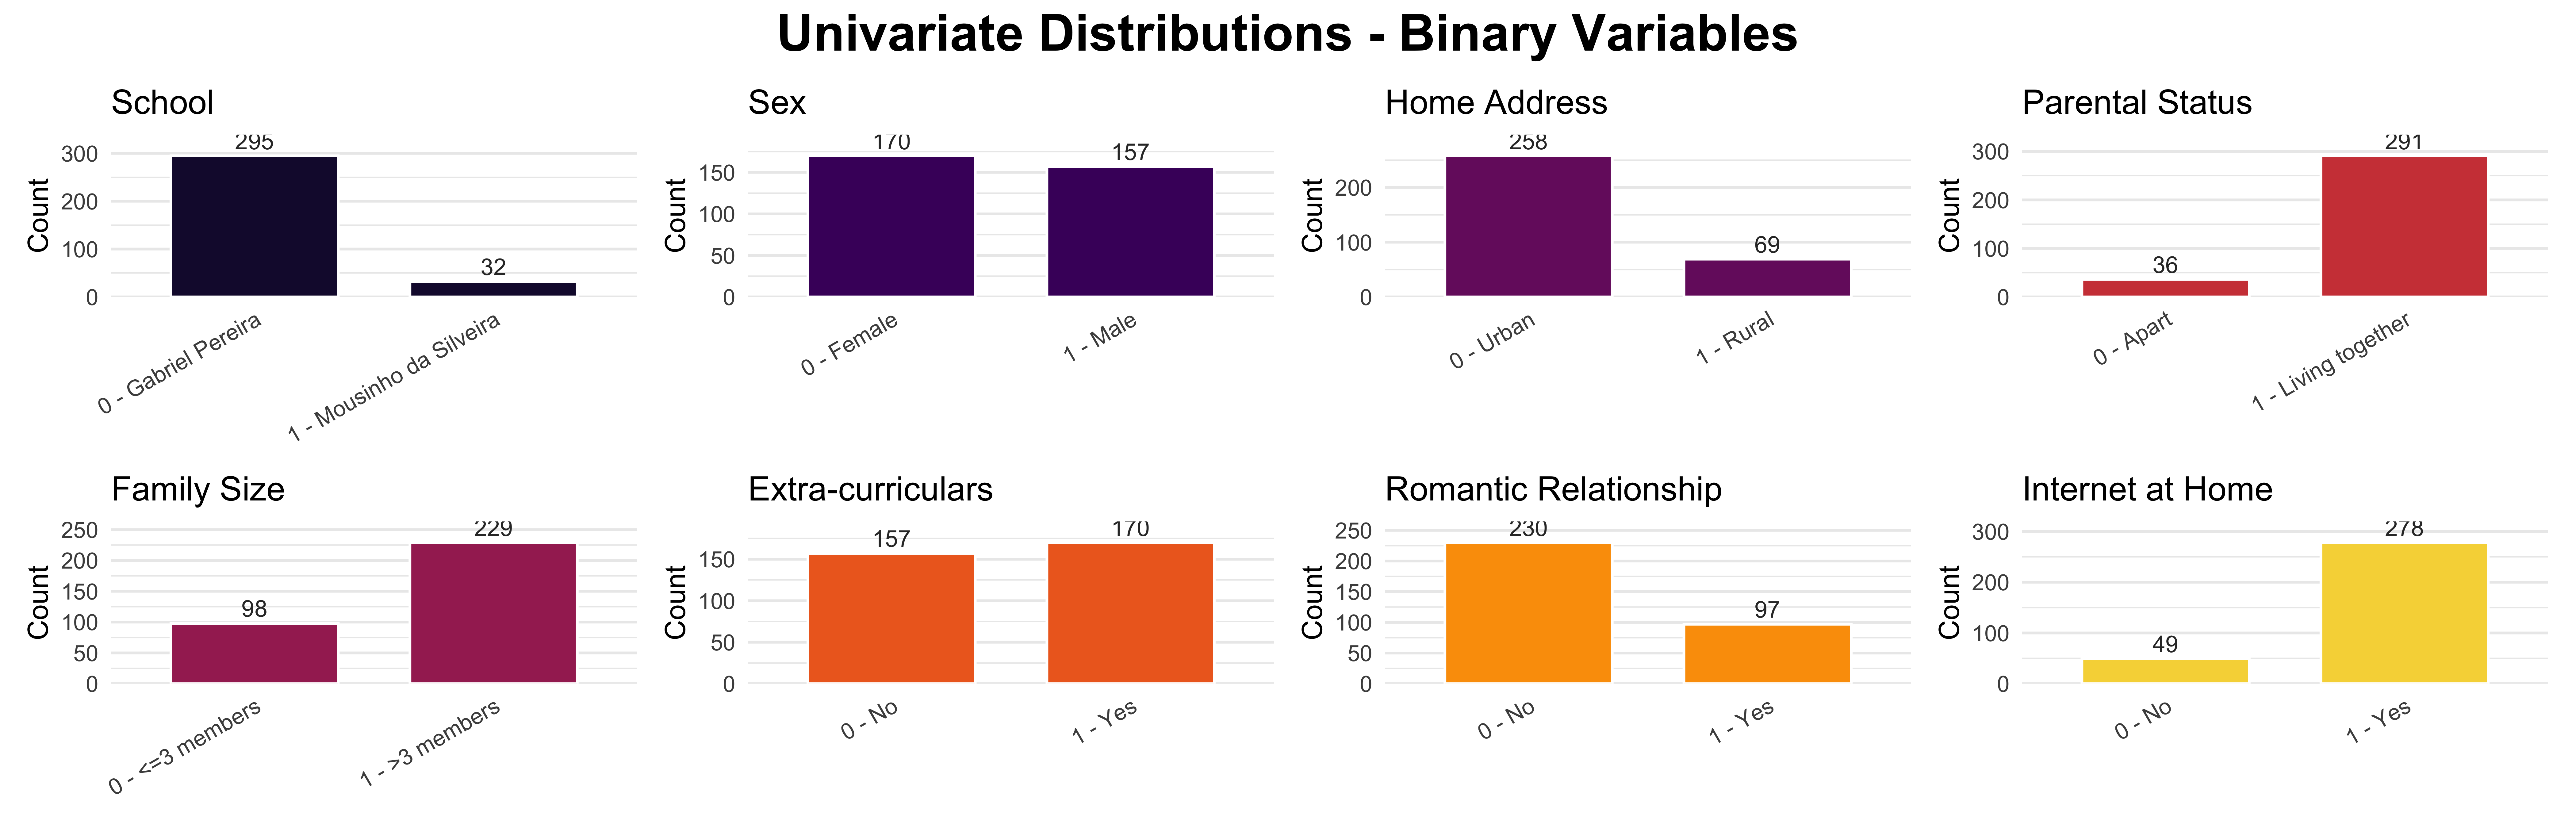
\includegraphics[width=\textwidth]{code_files/figure-html/ida_binary_plots-1.png}
\end{figure}

\newpage
\textbf{school}, the sample is heavily dominated by Gabriel Pereira, with only 32 students from Mousinho da Silveira. This imbalance is worth keeping in mind as the school coefficient will be estimated from a very small contrast group.

\vspace{0.2em}
\textbf{sex}, the split is nearly equal.

\vspace{0.2em}
\textbf{address}, the majority of students live in urban area, with rural students representing about a fifth of the sample --- both groups are sufficiently represented.

\vspace{0.2em}
\textbf{Pstatus and famsize}, both variables show imbalance in the same direction: most students come from larger families and from households where parents live together. The "Apart" category for Pstatus is particularly sparse, which may produce an unstable estimate --- we kept this in mind.

\vspace{0.2em}
\textbf{activities and romantic}, activities is nearly balanced. Romantic relationships are less common but still well-represented, with a little bit less than third of students reporting being in a relationship.

\vspace{0.2em}
\textbf{internet}, the large majority of students have internet access at home, leaving only 49 without. This imbalance is not extreme enough to require action, but we kept it in mind.



\subsection{IDA Screening: Multivariate Analysis}

In this subsection we summarize multivariate characteristics of the variables we selected. 


\subsubsection*{Stratification by Sex and School}
We performed stratification on two general variables, namely, by \textbf{sex} and by \textbf{school}. Stratification by all remaining variables was omitted to avoid inflating the report with uninformative visuals --- the correlation structure between predictors will be addressed more systematically in the subsequent correlation and redundancy analysis.

\begin{figure}[h!]
    \centering

    \begin{subfigure}[t]{0.495\textwidth}
        \centering
        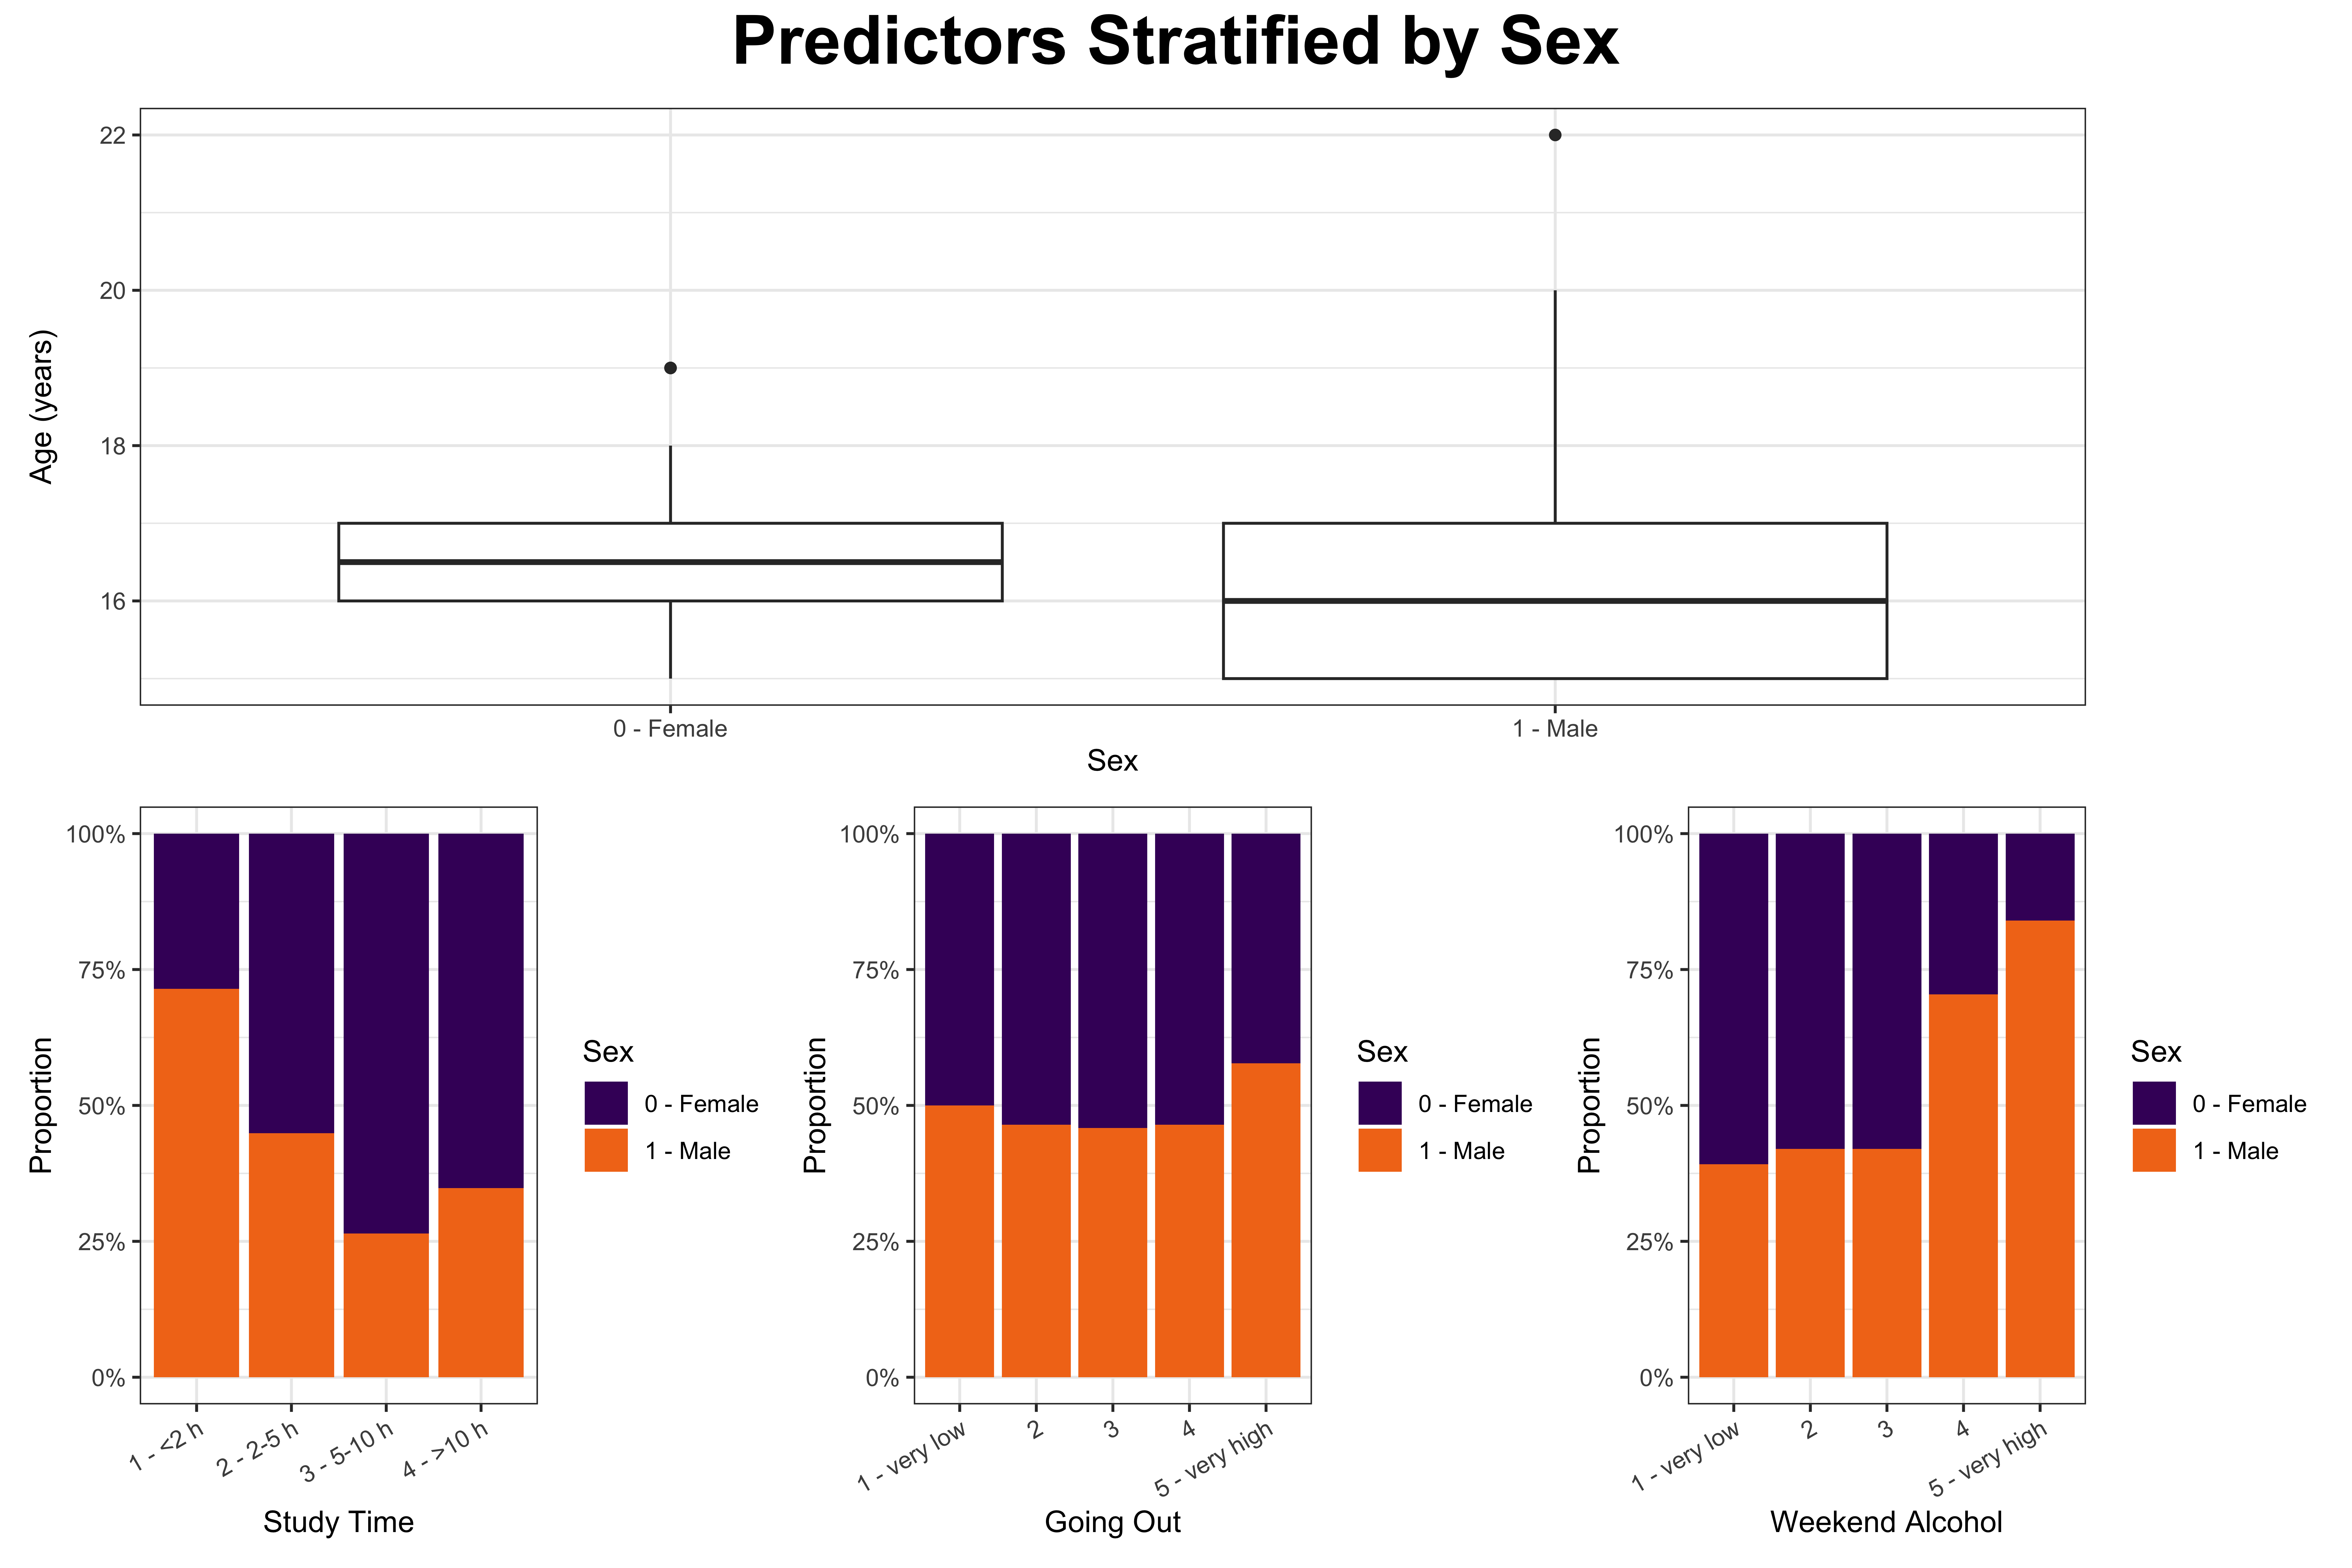
\includegraphics[width=\linewidth]{code_files/figure-html/ida_strat_sex_plots-1.png}
        \caption{Stratification by Sex}
    \end{subfigure}
    \hfill
    \begin{subfigure}[t]{0.495\textwidth}
        \centering
        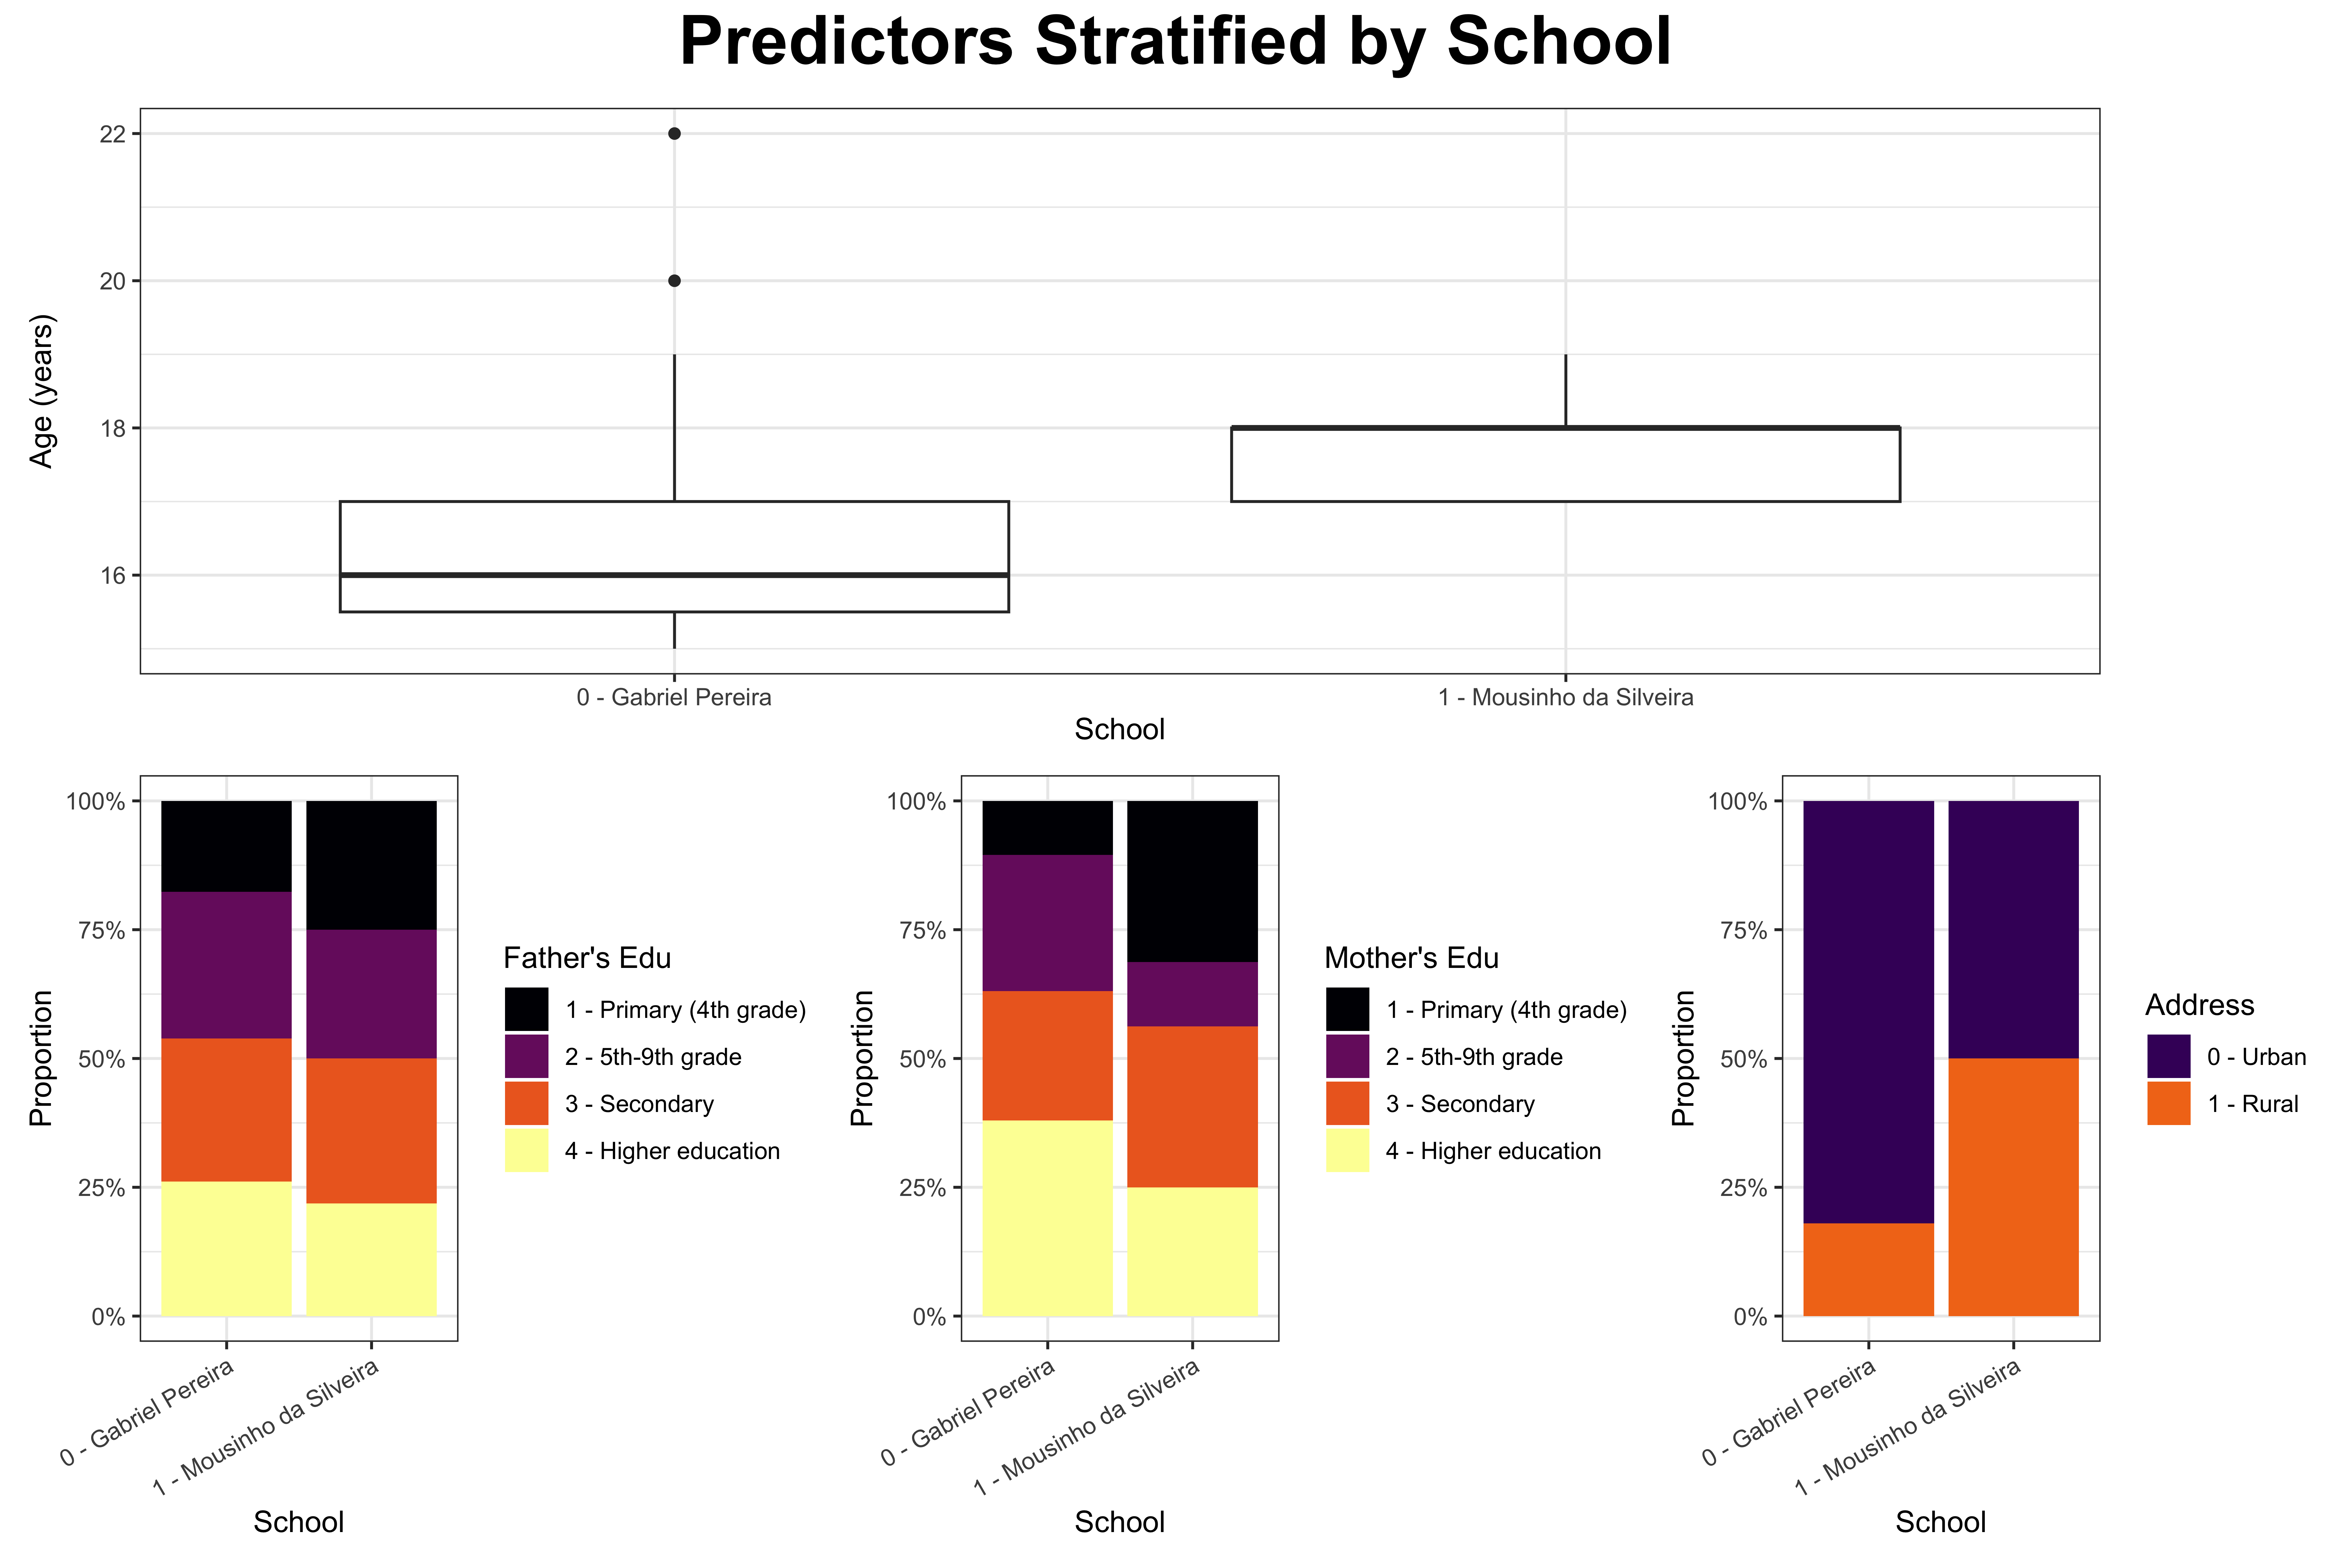
\includegraphics[width=\linewidth]{code_files/figure-html/ida_strat_school_plots-1.png}
        \caption{Stratification by School}
    \end{subfigure}

\end{figure}

Notable observations from the sex-based stratification suggest that female students tend to spend more time studying and consume smaller amounts of alcohol on weekends compared to male students in this sample, particularly at higher levels of consumption. In terms of age, female students are slightly older on average and exhibit less variability compared to male students.

\vspace{0.2em}

The school-based stratification shows that students from Mousinho da Silveira are generally older, and their parents --- particularly mothers --- have notably lower levels of formal education compared to those at Gabriel Pereira. There is also a clear geographic divide, with approximately half of Mousinho da Silveira students coming from rural areas, whereas Gabriel Pereira serves a predominantly urban population. Overall, Mousinho da Silveira reflects a student population facing more pronounced socioeconomic and environmental constraints.


\subsubsection*{Correlation Between All Predictors}

We now summarize the pairwise associations between all predictors using a Spearman correlation matrix with a heatmap. To ensure comparability across mixed data types (binary, ordinal, and continuous variables), all predictors are converted into a numeric representation. This step complements the univariate and stratified analyses.

\newpage
\begin{figure}[h!]
    \centering
    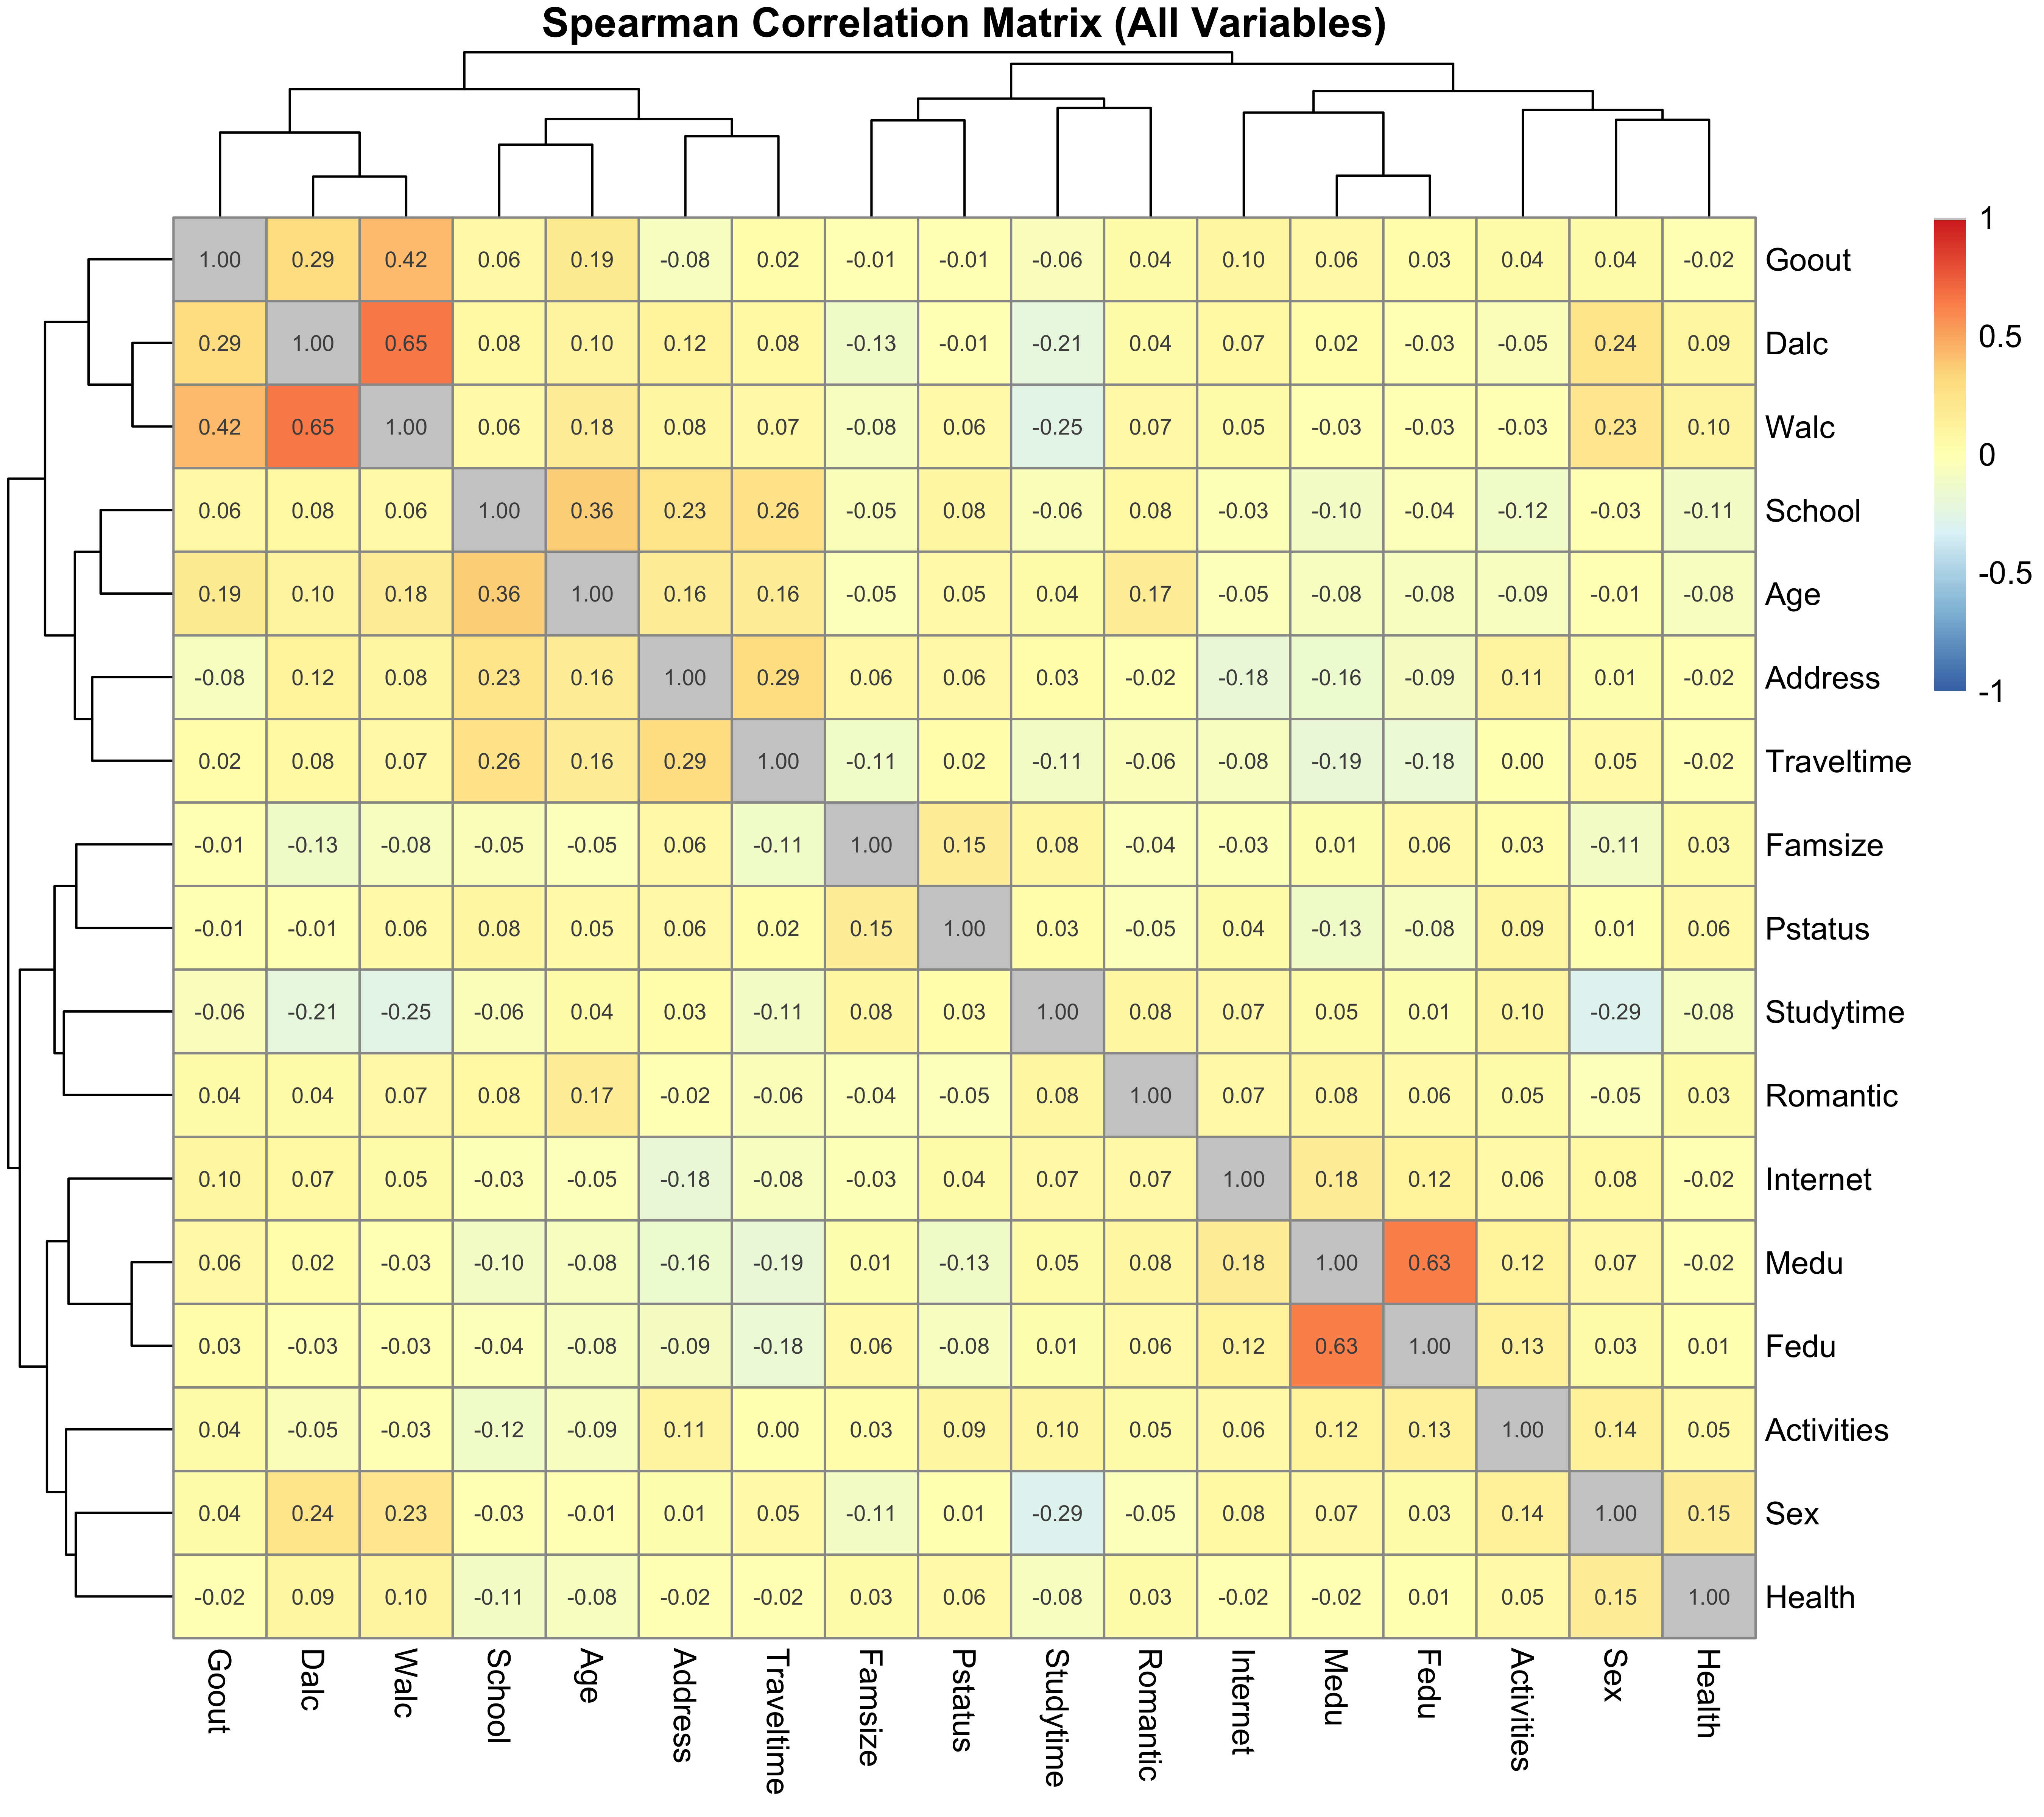
\includegraphics[width=0.8\textwidth]{code_files/figure-html/ida_heatmap_all-1.png}
\end{figure}

We observe some expected clusters. The strongest positive correlations are between Mother's Education (`Medu`) and Father's Education (`Fedu`), as well as between Workday Alcohol Consumption (`Dalc`) and Weekend Alcohol Consumption (`Walc`) - what we hypothesized in the beginning. There is also a notable positive association between `Walc` and `Goout` (similarly for `Dalc` and `Goout` but weaker) - which is expectable given that some of going out activities include alcohol consumption. Additionaly, there is a negative association between `studytime` and `sex` - the observation we made when performing stratification by sex. Additionally, note that Spearman correlation is used as a common ground for our mix of binary, ordinal, and continuous variables, rather than as the theoretically optimal measure for every pair.



\subsubsection*{Redundancy Analysis}

To make a final decision of keeping or not keeping all of the variables, we performed Redundancy Analysis.
Note that we set number of knots to zero to suppress spline transformations, as most predictors have only 4 ordinal levels --- too few to support non-linear fits. This principally reduces the redundancy analysis to a linear check, which gives information similar to multicollinearity we peformed in the previous subsection, but adds "directions" so we can understnad exactly which of the correlated variables can be explained more.

\vspace{0.5em} \noindent
\begin{tabularx}{\textwidth}{Xr Xr Xr Xr Xr Xr}
\hline
Variable & $R^2$ & Variable & $R^2$ & Variable & $R^2$ & Variable & $R^2$ & Variable & $R^2$ & Variable & $R^2$ \\
\hline
age        & 0.225 & school    & 0.244 & sex      & 0.207 & address   & 0.233 & famsize  & 0.096 & Pstatus   & 0.122 \\
Medu       & 0.455 & Fedu      & 0.432 & internet & 0.106 & health    & 0.095 & goout    & 0.262 & traveltime & 0.225 \\
activities & 0.126 & Dalc      & 0.484 & Walc     & 0.554 & studytime & 0.204 & romantic & 0.118 &           &       \\
\hline
\end{tabularx}

\vspace{0.5em}
The redundancy analysis showed that no variable exceeds the $R^2 = 0.9$ redundancy threshold, meaning no predictor can be linearly reconstructed from the remaining variables with sufficient precision to warrant automatic exclusion. The highest $R^2$ values belong to `Walc` (0.554) and `Dalc` (0.484), reflecting their shared alcohol-consption construct --- consistent with the correlation observed in the heatmap. `Medu` and `Fedu` follow at 0.455 and 0.432 respectively, again expected given their correlation, but well below the redundancy cutoff. All remaining variables have $R^2$ below 0.33, indicating they each contribute largely independent information. On these facts alone, no variable would be excluded --- however, the decisions were revisited in the IDA conclusions.



\subsection{IDA Conclusions}

Based on the screening, three sets of decisions are carried into model fitting.

\vspace{0.2em}
\textbf{Variable exclusion.} `Dalc` is dropped from the analytic models. This decision is not motivated by multicollinearity (which as we have seen is present, but not extreme), rather, the justification is distributional: most of students score at the lowest level, and after collapsing the sparse upper categories the variable would effectively reduce to a near-binary indicator. `Walc`, which is better spread across all five levels and captures the same underlying alcohol consumption construct, is thus kept as the sole alcohol consumption predictor.

\vspace{0.2em}
\textbf{Level recoding.} For `traveltime`, the top two levels ("30 min -- 1 h" and "\textgreater1 h") are merged into a single "\textgreater=30 min" category, as the original cell sizes (16 and 7 observations respectively) were too small to produce meaningful coefficient estimates.

\vspace{0.2em}
\textbf{Underrepresented categories.} Three binary variables show notable imbalance: `school` (only 32 students from Mousinho da Silveira), `Pstatus` (36 observations in "Apart" category), and `internet` (only 49 students without home access). These variables are kept in the models, as their imbalance is not severe enough to motivate exclusion and each carries plausible theoretical relevance. However, their coefficient estimates should be interpreted with caution --- the contrast groups are small, confidence intervals will be wide, and any effects may be unstable.




\section{Model Analysis}


\subsection{Fitted Coefficients + Interpretation}

\vspace{-1em}\noindent
\begin{minipage}[t]{0.49\textwidth}
\centering
\scriptsize
\textit{Mathematics --- Structural Model}\\[4pt]
\begin{tabularx}{\textwidth}{Xrrr}
\toprule
\textbf{Term} & \textbf{Est.} & \textbf{95\% CI} & \textbf{$p$} \\
\midrule
\textbf{Intercept}            & \textbf{16.52} & \textbf{[10.92,\ 22.12]} & \textbf{$<$0.001} \\
School: MS                    &  0.43 & [$-$0.88,\ 1.73] & 0.522 \\
\textbf{Sex: Male}            & \textbf{0.94} & \textbf{[0.23,\ 1.65]} & \textbf{0.010} \\
Age                           & $-$0.30 & [$-$0.63,\ 0.02] & 0.069 \\
Address: Rural                & $-$0.47 & [$-$1.40,\ 0.46] & 0.322 \\
Famsize: $>$3                 & $-$0.20 & [$-$0.98,\ 0.58] & 0.615 \\
Pstatus: Together             &  0.27 & [$-$0.88,\ 1.42] & 0.646 \\
Medu: 5th--9th vs Primary     &  1.12 & [$-$0.18,\ 2.42] & 0.090 \\
Medu: Secondary vs 5th--9th   &  0.21 & [$-$0.83,\ 1.24] & 0.693 \\
Medu: Higher vs Secondary     &  0.62 & [$-$0.36,\ 1.59] & 0.214 \\
Fedu: 5th--9th vs Primary     &  0.33 & [$-$0.78,\ 1.45] & 0.558 \\
Fedu: Secondary vs 5th--9th   & $-$0.72 & [$-$1.70,\ 0.28] & 0.156 \\
Fedu: Higher vs Secondary     &  0.93 & [$-$0.08,\ 1.94] & 0.071 \\
Travel: 15--30 vs $<$15 min   & $-$0.35 & [$-$1.20,\ 0.49] & 0.411 \\
Travel: $\geq$30 vs 15--30    &  0.02 & [$-$1.50,\ 1.54] & 0.982 \\
Internet: Yes                 &  0.19 & [$-$0.81,\ 1.19] & 0.710 \\
\textbf{Health}               & \textbf{$-$0.28} & \textbf{[$-$0.53,\ $-$0.03]} & \textbf{0.030} \\
\bottomrule
\end{tabularx}
\end{minipage}
\hfill
\begin{minipage}[t]{0.49\textwidth}
\centering
\scriptsize
\textit{Portuguese --- Structural Model}\\[4pt]
\begin{tabularx}{\textwidth}{Xrrr}
\toprule
\textbf{Term} & \textbf{Est.} & \textbf{95\% CI} & \textbf{$p$} \\
\midrule
\textbf{Intercept}            & \textbf{10.29} & \textbf{[5.96,\ 14.61]} & \textbf{$<$0.001} \\
School: MS                    & $-$0.28 & [$-$1.29,\ 0.73] & 0.582 \\
\textbf{Sex: Male}            & \textbf{$-$0.97} & \textbf{[$-$1.52,\ $-$0.42]} & \textbf{$<$0.001} \\
Age                           &  0.23 & [$-$0.02,\ 0.48] & 0.067 \\
Address: Rural                & $-$0.61 & [$-$1.33,\ 0.11] & 0.096 \\
Famsize: $>$3                 & $-$0.05 & [$-$0.65,\ 0.56] & 0.878 \\
Pstatus: Together             & $-$0.15 & [$-$1.04,\ 0.74] & 0.745 \\
Medu: 5th--9th vs Primary     &  0.23 & [$-$0.78,\ 1.23] & 0.657 \\
Medu: Secondary vs 5th--9th   &  0.25 & [$-$0.55,\ 1.05] & 0.542 \\
\textbf{Medu: Higher vs Secondary} & \textbf{0.88} & \textbf{[0.13,\ 1.64]} & \textbf{0.022} \\
Fedu: 5th--9th vs Primary     &  0.25 & [$-$0.61,\ 1.11] & 0.568 \\
Fedu: Secondary vs 5th--9th   & $-$0.54 & [$-$1.30,\ 0.23] & 0.167 \\
Fedu: Higher vs Secondary     &  0.64 & [$-$0.14,\ 1.42] & 0.109 \\
Travel: 15--30 vs $<$15 min   & $-$0.06 & [$-$0.71,\ 0.60] & 0.862 \\
Travel: $\geq$30 vs 15--30    & $-$0.27 & [$-$1.45,\ 0.90] & 0.650 \\
Internet: Yes                 &  0.03 & [$-$0.74,\ 0.81] & 0.935 \\
\textbf{Health}               & \textbf{$-$0.23} & \textbf{[$-$0.42,\ $-$0.03]} & \textbf{0.023} \\
\bottomrule
\end{tabularx}
\end{minipage}


\vspace{0.5em}
\noindent
\begin{minipage}[t]{0.49\textwidth}
\centering
\scriptsize
\textit{Mathematics --- Full Model}\\[4pt]
\begin{tabularx}{\textwidth}{Xrrr}
\toprule
\textbf{Term} & \textbf{Est.} & \textbf{95\% CI} & \textbf{$p$} \\
\midrule
\textbf{Intercept}            & \textbf{17.02} & \textbf{[11.51,\ 22.53]} & \textbf{$<$0.001} \\
School: MS                    &  0.53 & [$-$0.75,\ 1.80] & 0.416 \\
\textbf{Sex: Male}            & \textbf{1.27} & \textbf{[0.54,\ 2.01]} & \textbf{$<$0.001} \\
Age                           & $-$0.17 & [$-$0.49,\ 0.16] & 0.308 \\
Address: Rural                & $-$0.79 & [$-$1.72,\ 0.13] & 0.091 \\
Famsize: $>$3                 & $-$0.38 & [$-$1.14,\ 0.38] & 0.321 \\
Pstatus: Together             &  0.10 & [$-$1.02,\ 1.22] & 0.862 \\
Medu: 5th--9th vs Primary     &  0.82 & [$-$0.44,\ 2.08] & 0.201 \\
Medu: Secondary vs 5th--9th   &  0.28 & [$-$0.72,\ 1.29] & 0.581 \\
Medu: Higher vs Secondary     &  0.57 & [$-$0.38,\ 1.52] & 0.236 \\
Fedu: 5th--9th vs Primary     &  0.38 & [$-$0.69,\ 1.46] & 0.483 \\
Fedu: Secondary vs 5th--9th   & $-$0.65 & [$-$1.61,\ 0.31] & 0.183 \\
Fedu: Higher vs Secondary     &  0.97 & [$-$0.01,\ 1.94] & 0.053 \\
Travel: 15--30 vs $<$15 min   & $-$0.41 & [$-$1.22,\ 0.41] & 0.328 \\
Travel: $\geq$30 vs 15--30    &  0.47 & [$-$1.01,\ 1.96] & 0.530 \\
Internet: Yes                 &  0.17 & [$-$0.81,\ 1.14] & 0.735 \\
\textbf{Health}               & \textbf{$-$0.28} & \textbf{[$-$0.52,\ $-$0.03]} & \textbf{0.026} \\
\textbf{Goout}                & \textbf{$-$0.38} & \textbf{[$-$0.72,\ $-$0.03]} & \textbf{0.033} \\
Activities: Yes               &  0.12 & [$-$0.59,\ 0.82] & 0.748 \\
Walc                          & $-$0.30 & [$-$0.62,\ 0.01] & 0.057 \\
Studytime: 2--5 vs $<$2 h     & $-$0.52 & [$-$1.38,\ 0.33] & 0.229 \\
\textbf{Studytime: 5--10 vs 2--5 h} & \textbf{1.52} & \textbf{[0.53,\ 2.52]} & \textbf{0.003} \\
Studytime: $>$10 vs 5--10 h   &  0.27 & [$-$1.27,\ 1.80] & 0.733 \\
Romantic: Yes                 & $-$0.28 & [$-$1.04,\ 0.48] & 0.471 \\
\bottomrule
\end{tabularx}
\end{minipage}
\hfill
\begin{minipage}[t]{0.49\textwidth}
\centering
\scriptsize
\textit{Portuguese --- Full Model}\\[4pt]
\begin{tabularx}{\textwidth}{Xrrr}
\toprule
\textbf{Term} & \textbf{Est.} & \textbf{95\% CI} & \textbf{$p$} \\
\midrule
\textbf{Intercept}            & \textbf{10.34} & \textbf{[6.14,\ 14.54]} & \textbf{$<$0.001} \\
School: MS                    & $-$0.09 & [$-$1.06,\ 0.89] & 0.864 \\
\textbf{Sex: Male}            & \textbf{$-$0.61} & \textbf{[$-$1.17,\ $-$0.05]} & \textbf{0.033} \\
\textbf{Age}                  & \textbf{0.35} & \textbf{[0.10,\ 0.60]} & \textbf{0.006} \\
\textbf{Address: Rural}       & \textbf{$-$0.94} & \textbf{[$-$1.65,\ $-$0.24]} & \textbf{0.009} \\
Famsize: $>$3                 & $-$0.13 & [$-$0.70,\ 0.45] & 0.669 \\
Pstatus: Together             & $-$0.28 & [$-$1.14,\ 0.57] & 0.515 \\
Medu: 5th--9th vs Primary     &  0.06 & [$-$0.90,\ 1.02] & 0.899 \\
Medu: Secondary vs 5th--9th   &  0.33 & [$-$0.44,\ 1.09] & 0.402 \\
\textbf{Medu: Higher vs Secondary} & \textbf{0.83} & \textbf{[0.11,\ 1.55]} & \textbf{0.025} \\
Fedu: 5th--9th vs Primary     &  0.24 & [$-$0.58,\ 1.06] & 0.571 \\
Fedu: Secondary vs 5th--9th   & $-$0.63 & [$-$1.36,\ 0.11] & 0.094 \\
\textbf{Fedu: Higher vs Secondary} & \textbf{0.76} & \textbf{[0.01,\ 1.50]} & \textbf{0.047} \\
Travel: 15--30 vs $<$15 min   & $-$0.06 & [$-$0.69,\ 0.56] & 0.843 \\
Travel: $\geq$30 vs 15--30    &  0.18 & [$-$0.95,\ 1.31] & 0.755 \\
Internet: Yes                 &  0.03 & [$-$0.72,\ 0.77] & 0.947 \\
\textbf{Health}               & \textbf{$-$0.22} & \textbf{[$-$0.41,\ $-$0.03]} & \textbf{0.022} \\
\textbf{Goout}                & \textbf{$-$0.43} & \textbf{[$-$0.69,\ $-$0.16]} & \textbf{0.002} \\
Activities: Yes               &  0.44 & [$-$0.09,\ 0.98] & 0.106 \\
Walc                          & $-$0.17 & [$-$0.41,\ 0.07] & 0.152 \\
Studytime: 2--5 vs $<$2 h     &  0.59 & [$-$0.06,\ 1.24] & 0.076 \\
\textbf{Studytime: 5--10 vs 2--5 h} & \textbf{0.84} & \textbf{[0.08,\ 1.60]} & \textbf{0.030} \\
Studytime: $>$10 vs 5--10 h   & $-$0.03 & [$-$1.20,\ 1.14] & 0.962 \\
Romantic: Yes                 & $-$0.26 & [$-$0.84,\ 0.32] & 0.380 \\
\bottomrule
\end{tabularx}
\end{minipage}


\vspace{-1em}
\paragraph{Mathematics --- Structural Model}

Only two predictors reach statistical significance. \textbf{Sex} is the strongest and most consistent signal: males score +0.94 on average (95\% CI: 0.23, 1.65). \textbf{Health} is also significant but counterintuitive in direction: each unit increase (better reported health) is associated with a \textit{decrease} of 0.28 (95\% CI: $-0.53$, $-0.03$). All remaining predictors are non-significant, indicating that environmental background alone explains very little variation in mathematics performance. The intercept is not interpretable: due to successive difference contrasts, it represents an average across factor levels rather than any meaningful student profile.


\paragraph{Mathematics --- Full Model}

\textbf{Sex} remains significant and increases to +1.27 (95\% CI: 0.54, 2.01). This widening gap is somewhat counterintuitive: although females were observed to study more (IDA), controlling for study time actually enlarges the gap, implying that study behavior was partially offsetting rather than explaining the underlying difference. \textbf{Health} remains stable ($-0.28$, 95\% CI: $-0.52$, $-0.03$), suggesting that the effect is not driven by simple social confounding (with the explanation instead linked to non-linearity).

\vspace{0.2em}
Among behavioral predictors, \textbf{study time} shows the clearest and most interpretable effect, though with a non-monotone pattern: the contrast 5--10h vs 2--5h yields +1.52 (95\% CI: 0.53, 2.52), while the lowest and highest contrasts remain non-significant. This points to a threshold effect, where moving from moderate to substantial study time matters, but additional effort beyond that does not yield further gains.

\vspace{0.2em}
\textbf{Going out} is the only other clearly significant behavioral predictor ($-0.38$, 95\% CI: $-0.72$, $-0.03$). \textbf{Weekend alcohol} is borderline ($-0.30$, 95\% CI: $-0.62$, 0.01) and is therefore not interpreted as a firm finding, although its direction is consistent with the broader pattern. \textbf{Romantic relationship} and \textbf{activities} are both non-significant, with estimates effectively indistinguishable from zero.


\paragraph{Portuguese --- Structural Model}

\textbf{Health} is again significant and negative ($-0.23$, 95\% CI: $-0.41$, $-0.22$), mirroring the mathematics result. \textbf{Sex} also remains a clear structural signal, but with reversed direction: females score +0.97 (95\% CI: 0.42, 1.52), in contrast to males performing better in mathematics.

\vspace{0.2em}
Parental education is largely non-significant, with one notable exception: the contrast between higher and secondary maternal education (+0.88, 95\% CI: 0.13, 1.64). This suggests a limited but specific benefit at the upper end of the education distribution. All other structural variables --- school, family size, parental status, travel time, internet, and address --- remain non-significant.


\paragraph{Portuguese --- Full Model}

\textbf{Sex} remains significant but decreases to +0.61 (95\% CI: 0.05, 1.17), suggesting behavioral differences explain part of the observed gap. \textbf{Age} becomes significant (+0.35 per year, 95\% CI: 0.1, 0.6), which was not the case in the structural model; this likely reflects a suppression effect from behavioral variables correlated with age. \textbf{Address} also becomes significant: rural students score $-0.94$ on average (95\% CI: $-1.65$, $-0.24$), a pattern not observed in mathematics. \textbf{Health} remains consistently negative ($-0.22$, 95\% CI: $-0.41$, $-0.03$).

\vspace{0.2em}
Mother’s education (higher vs secondary) remains significant (+0.83, 95\% CI: 0.11, 1.55), and father’s education at the same contrast also reaches significance (+0.76, $p = 0.047$), indicating a somewhat stronger parental education gradient than in mathematics.

\vspace{0.2em}
Among behavioral predictors, \textbf{going out} is again significant ($-0.43$, 95\% CI: $-0.69$, $-0.16$), closely matching the magnitude and direction seen in mathematics. \textbf{Study time} shows the same non-monotone threshold structure: 5--10h vs 2--5h yields +0.84 (95\% CI: 0.01, 1.6), while other contrasts remain non-significant, though the overall effect size is smaller than in mathematics. \textbf{Weekend alcohol}, \textbf{romantic relationship}, and \textbf{activities} remain non-significant, reinforcing the consistency across subjects.

\vspace{0.2em}
Overall, the comparative picture is clear: structural effects are generally weak; the sex gap persists but reverses direction across subjects; and behavioral effects concentrate primarily in study intensity and social activity. Portuguese differs in showing a stronger high-end parental education effect, a rural penalty absent in mathematics, and an age effect that only becomes visible after controlling for behavior.



\subsection{Model Comparison}


In this subsection we compare the predictive power of the models.

\vspace{-0.5em}
\begin{table}[h!]
\centering
\footnotesize
\begin{tabularx}{\textwidth}{lrrrrrrr}
\toprule
\textbf{Model (Subject)} & \textbf{AIC} & \textbf{RMSE} & \textbf{MAE} & \textbf{CV-RMSE} & \textbf{CV-MAE} & \textbf{$R^2$} & \textbf{Adj.\ $R^2$} \\
\midrule
Structural (Math) & 1{,}698.40 & 3.07 & 2.48 & 3.24 & 2.62 & 0.114 & 0.068 \\
Full (Math)       & 1{,}678.27 & 2.92 & 2.38 & 3.15 & 2.57 & 0.202 & 0.141 \\
\midrule
Structural (Port.) & 1{,}529.66 & 2.37 & 1.86 & 2.52 & 1.96 & 0.139 & 0.094 \\
Full (Port.)       & 1{,}500.87 & 2.22 & 1.75 & 2.41 & 1.90 & 0.244 & 0.187 \\
\bottomrule
\end{tabularx}
\end{table}

\vspace{-0.5em}
Across both subjects, the full model outperforms the structural model on every metric. The AIC drops by around 20 and 29 points, for Mathematics and Portuguese. Thus, the behavioral predictors justify their inclusion even after accounting for the added complexity.
The clearest way to see the gain is through Adj. $R^2$: it roughly doubles in both subjects, from 0.068 to 0.141 in Mathematics and from 0.094 to 0.187 in Portuguese. This directly answers the core research question --- personal agency variables do add explanatory power beyond structural constraints, and the contribution is substantial relative to what the structural model achieves on its own. Portuguese shows a slightly larger gain overall, consistent with the stronger and more consistent signals we observed in the interpretation.

\vspace{0.2em}
In terms of actual prediction accuracy, the CV-RMSE provides the more honest comparison. The full model improves on the structural model in both subjects: CV-RMSE drops from 3.24 to 3.15 in Mathematics and from 2.52 to 2.41 in Portuguese, with CV-MAE showing the same direction. That said, the absolute prediction errors remain large: the best-performing model, the full Portuguese model, still carries a CV-RMSE of 2.41, meaning a typical out-of-sample prediction error of just under two and a half grade points on a 1--20 scale. So while the full model is the better model by every criterion, neither model predicts grades particularly well in absolute terms. An Adj. $R^2$ of 0.187 and 0.141 means roughly 80\% of the variation in Portuguese grades --- and nearly 86\% in Mathematics --- is left unexplained.


\subsection{Model Diagnostics}
In this subsections we discuss how reliable are the observations we made.

\begin{figure}[h!]
    \centering

    \begin{subfigure}[t]{0.495\textwidth}
        \centering
        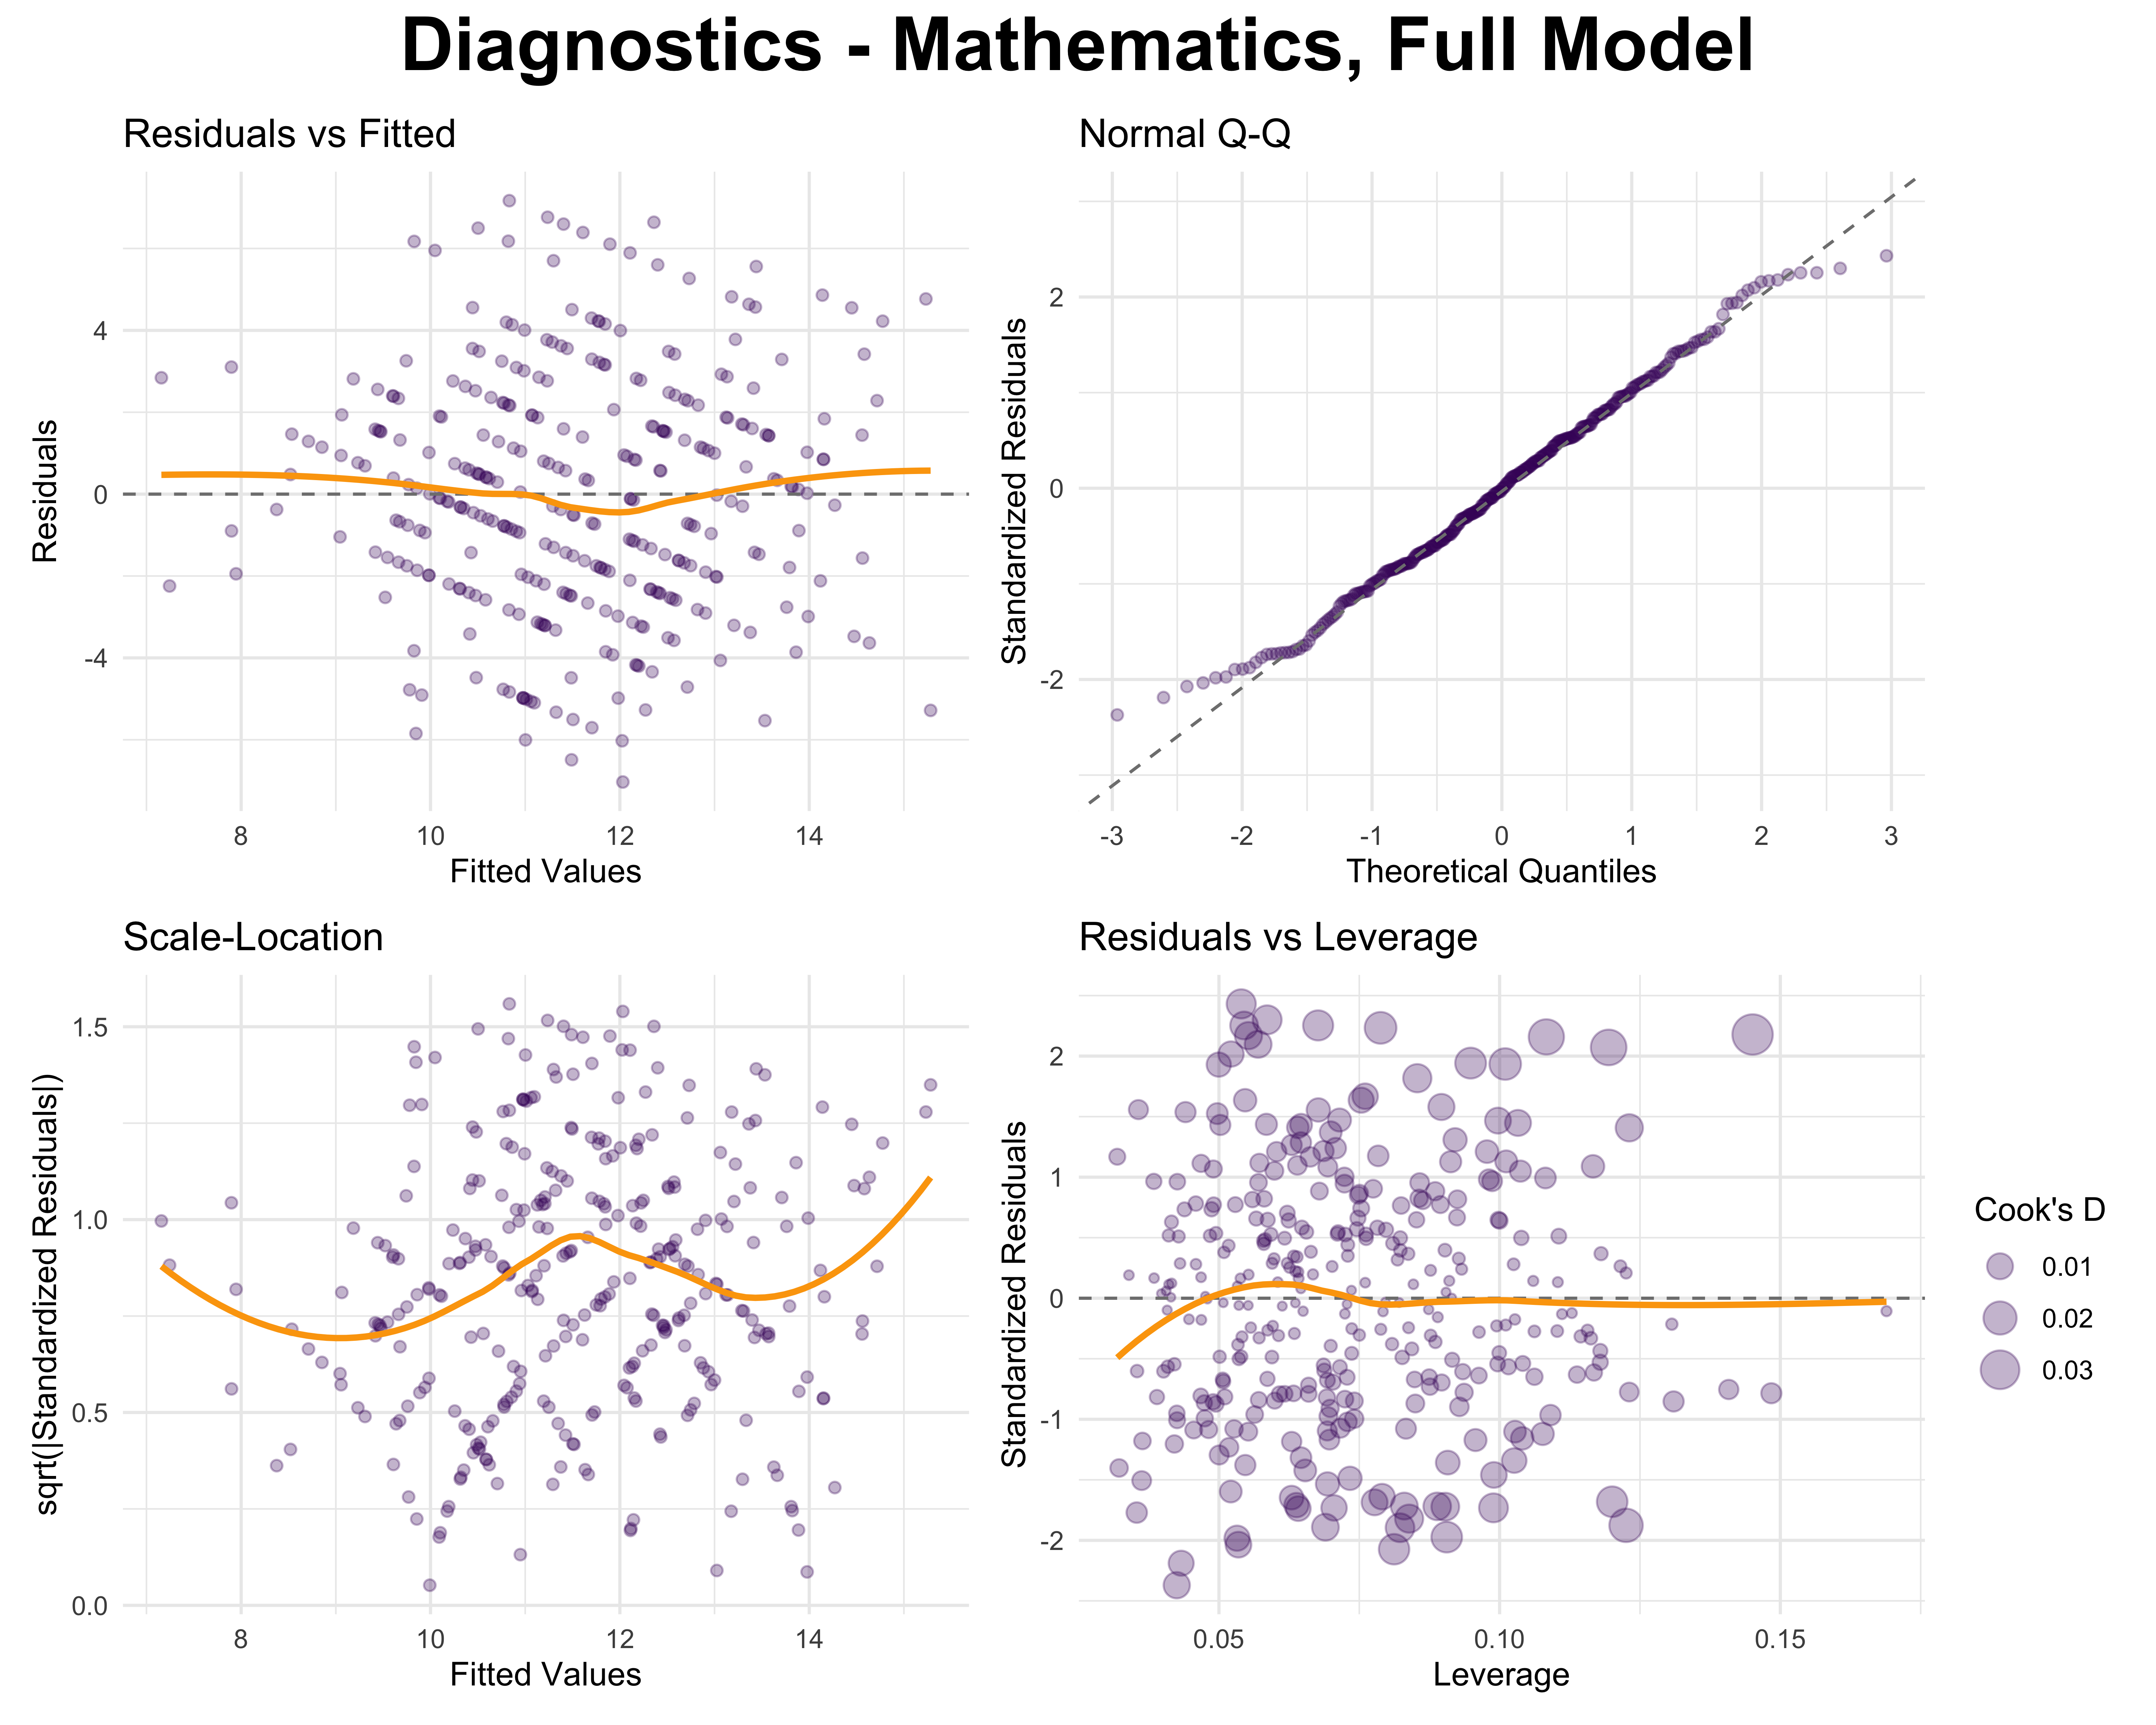
\includegraphics[width=\linewidth]{code_files/figure-html/diag_mat_full-1.png}
        \caption{Mathematics --- Full Model}
    \end{subfigure}
    \hfill
    \begin{subfigure}[t]{0.495\textwidth}
        \centering
        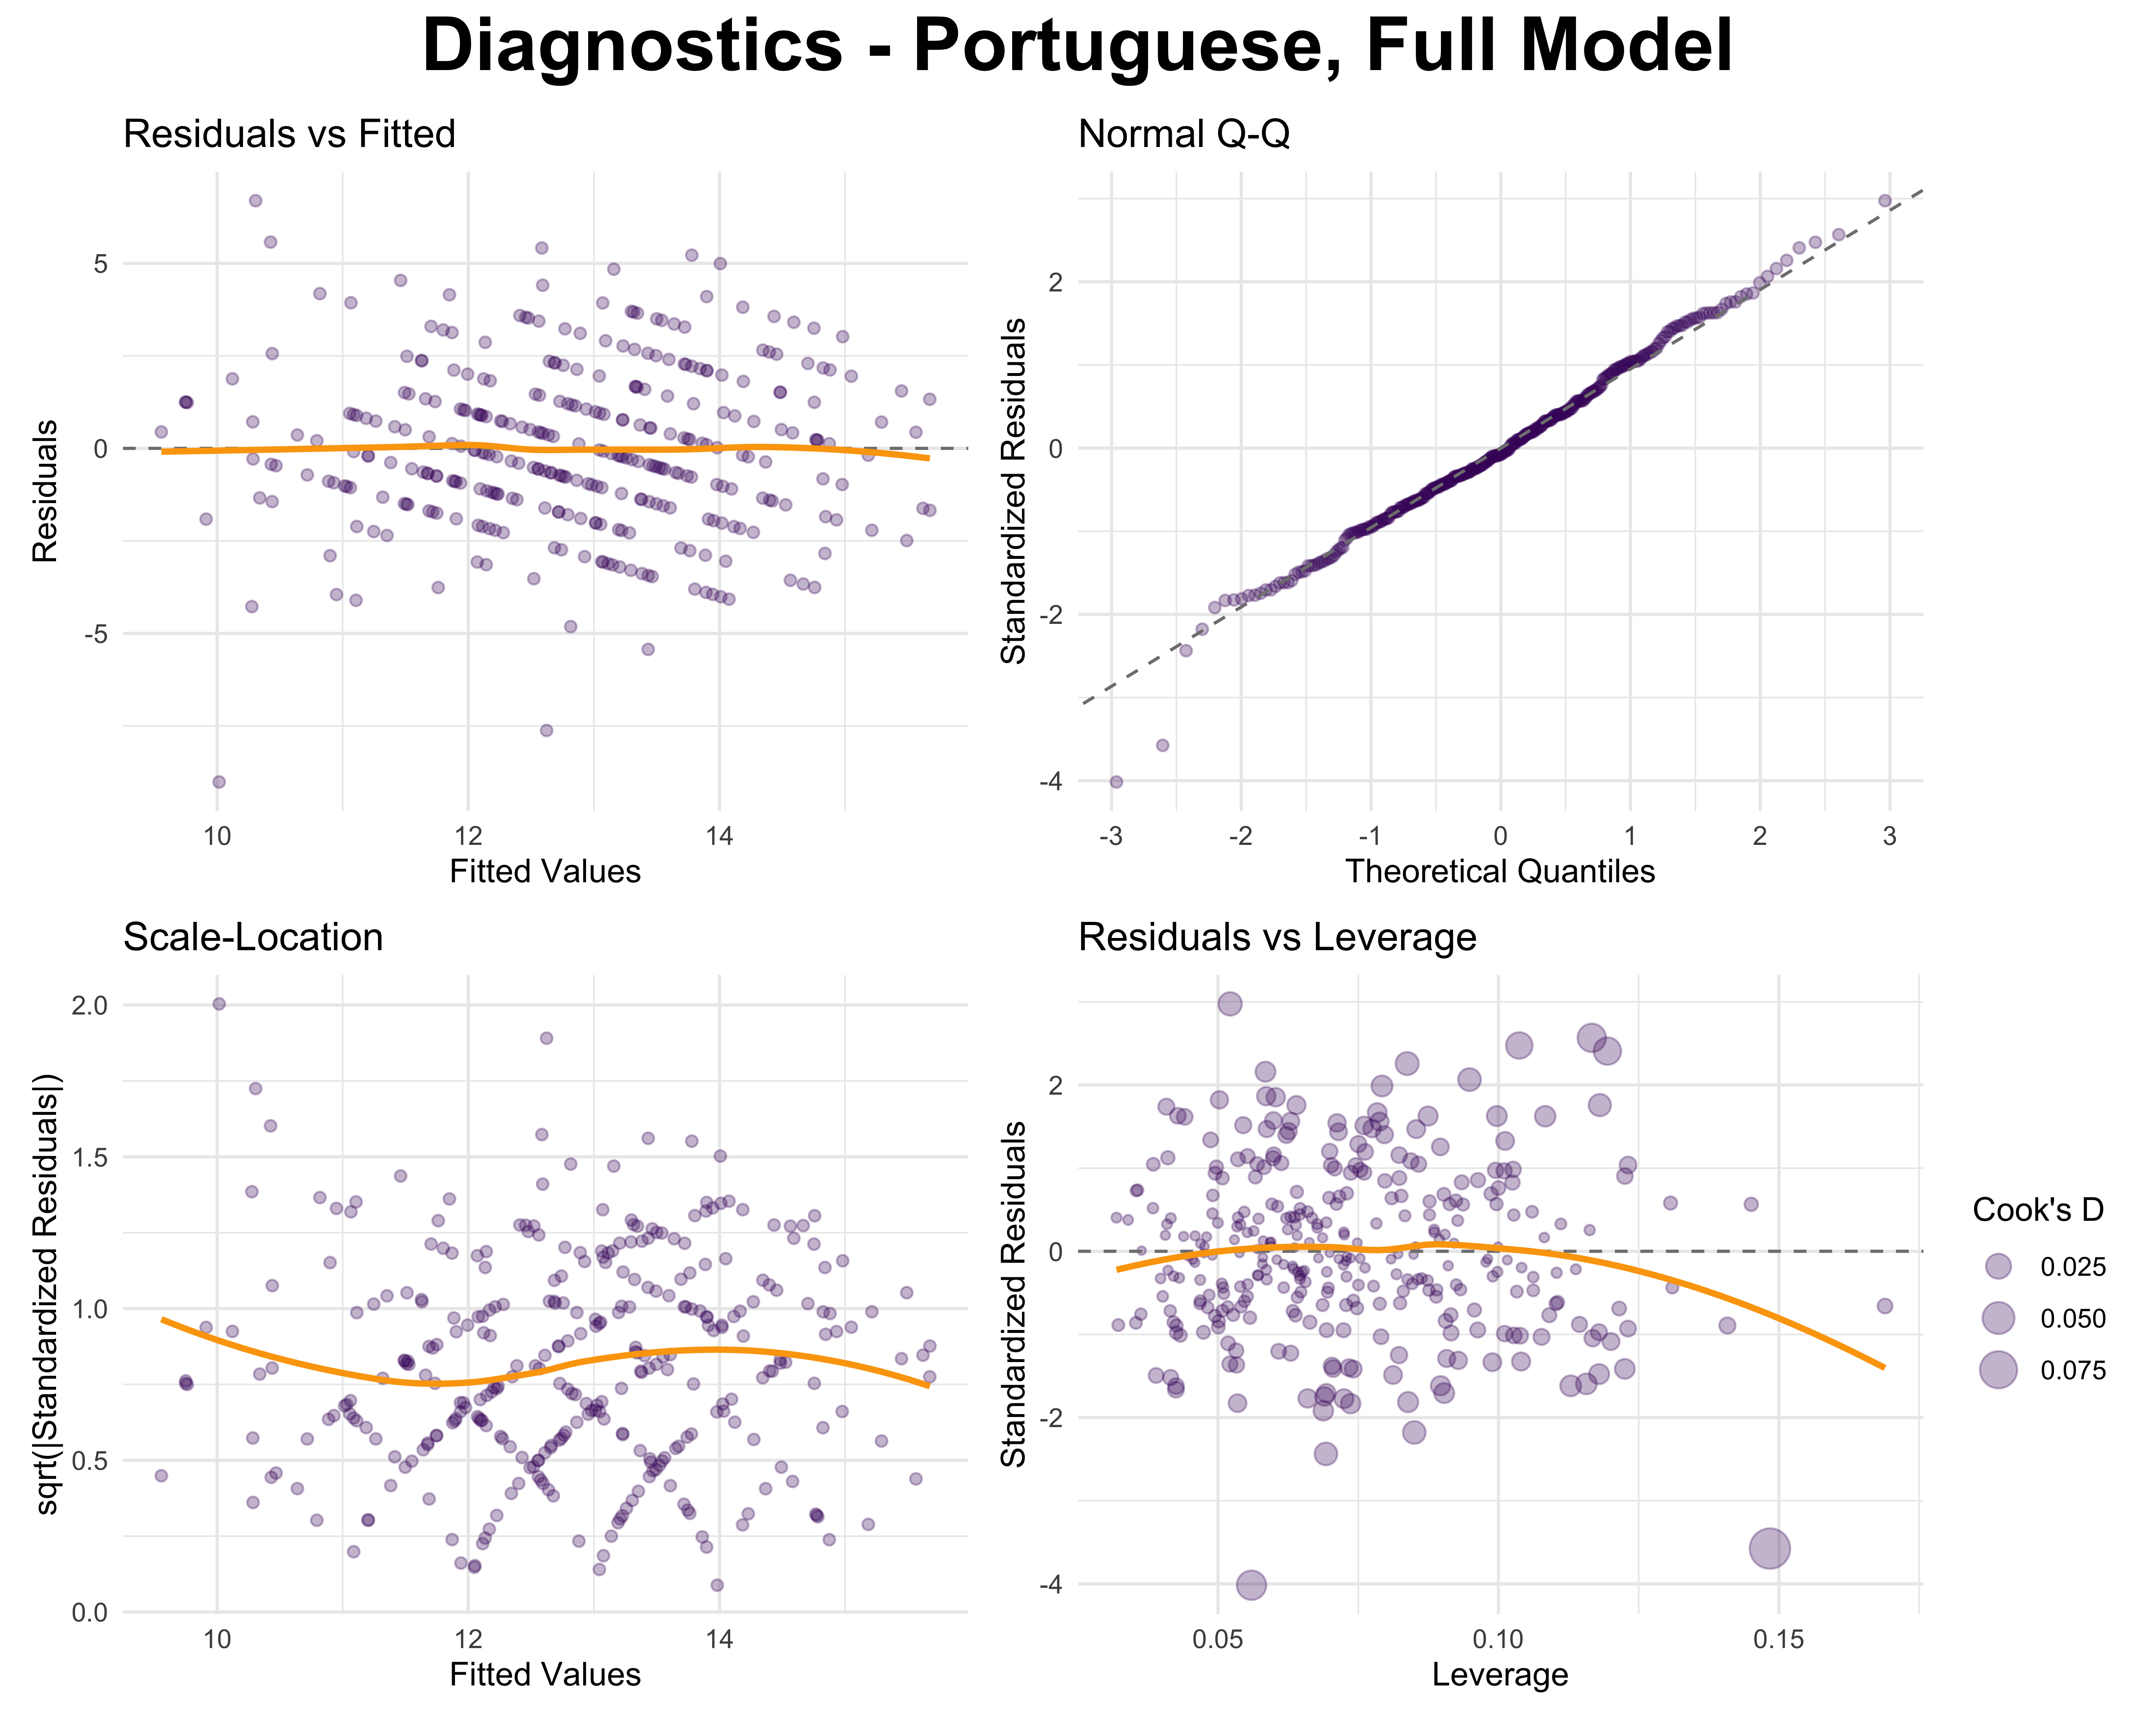
\includegraphics[width=\linewidth]{code_files/figure-html/diag_por_full-1.png}
        \caption{Portuguese --- Full Model}
    \end{subfigure}

\end{figure}

\vspace{-1em}
The diagnostic plots for both full models look healthy overall, with no severe violations of the core OLS assumptions. The residuals vs fitted plots show no obvious non-linearity in either subject, with the loess line sitting close to zero across the fitted range. The Q-Q plots confirm approximate normality of residuals in both cases, with only minor tail deviations in Mathematics. The scale-location plots show some variance instability in Mathematics suggesting mild heteroscedasticity, which means confidence intervals may be slightly optimistic and borderline results such as weekend alcohol should be treated with some caution. For Portuguese, the main thing to flag is a single high-leverage point with a noticeably larger Cook's D than the rest of the sample --- this is almost certainly the student with a final grade of 1 noted in the IDA. Their influence on the Portuguese estimates is limited but not negligible. Overall, we think that the models are reliable enough to support the interpretations made.



\subsection{Non-Linear Relationships}
\label{sec:nonlinear}

In this subsection we explore non-linear relationships of predictors with the outcome.

\begin{figure}[h!]
    \centering

    \begin{subfigure}[t]{0.495\textwidth}
        \centering
        \includegraphics[width=\linewidth]{code_files/figure-html/nonlinear_check-1.png}
    \end{subfigure}
    \hfill
    \begin{subfigure}[t]{0.495\textwidth}
        \centering
        \includegraphics[width=\linewidth]{code_files/figure-html/nonlinear_check_por-1.png}
    \end{subfigure}

\end{figure}

\vspace{-1em}
For the ordinal predictors encoded with successive difference contrasts --- `studytime`, `Medu`, `Fedu`, and `traveltime` --- the question of non-linearity is already addressed by the model specification itself. Each level transition receives its own coefficient, so the model is not forced to assume a linear step across categories. The interpretation sections already highlighted the most notable example of this: the non-monotone pattern in `studytime`, where the meaningful grade gain is present only at the 2--5 h to 5--10 h jump.

\vspace{0.2em}
The variables that were not checked are `health`, `goout`, and `Walc`, which were treated as strictly linear numeric predictors, and `age`. For these, we examine the relationship with the final grade graphically.

\vspace{0.2em}
For \textbf{health} in both Mathematics and Portugues, the pattern is non-monotone --- grades drop at level 3 (good health), and then go up. The negative linear coefficient in the model is therefore not something meaningful. For \textbf{going out} and \textbf{weekend alcohol}, the relationship seem to be relatively linear (there are deviations, `goout` has a jump from very low to low; but we think they are negligible given the significance and results being consistent with the expectations). For \textbf{age}, the loess and linear fits are very close for Mathematics, but for Portuguese we see a drastic drop at the right tail --- which is driven by outlier with grade 5.

\vspace{0.2em}
As a consequence, the most defensible correction would be for health (and maybe goout) to encode them as ordered factor with successive difference contrasts, as was done for studytime. However, as we discussed in the analysis plan this yields 4 (8) more coefficients, which we were not sure we could afford with this sample size; if we decided to encode all of the ordinal factors in this way, we would overwhelm the model --- so we should have treated some of the ordinals as numeric anyway --- and we did not expect that health has a non-linear pattern.

\vspace{0.2em}
But again, looking at it retrospectively, the health should have been recoded; and it would most likely remove or explain our finding of negative association with the final grade when treated as just numeric.




\section{Conclusion}
\label{sec:conclusion}

This study looks at whether personal agency --- defined as student-driven behavioral choices --- helps predict academic success in Portuguese and Mathematics, beyond structural and environmental factors. The short answer is yes, but the effect is modest and comes with some important notes.

\vspace{0.2em}
In both subjects, the full model performed better than the structural model on every measure. Adjusted $R^2$ roughly doubled, and AIC dropped by about 20 points. The behavioral patterns were clear: spending more time \textbf{going out} was linked to lower grades, while increasing \textbf{study time} from moderate (2--5 hours) to higher levels (5--10 hours) per week led to the largest improvement in grades. These patterns were consistent across subjects and models, which makes them more convincing.

\vspace{0.2em}
Structural variables, on the other hand, mostly did not show strong effects. Family background, parental education, travel time, and internet access had little independent impact. The only small exception was \textbf{parental education}, which showed some effect at higher levels in Portuguese, but not in Mathematics.

\vspace{0.2em}
Among the control variables, \textbf{sex} showed the most consistent pattern. It was important in all models and flipped between subjects --- male students did better in Mathematics, while female students did better in Portuguese. What is interesting is how this changed after adding behavioral factors. In Portuguese, the female advantage became smaller, suggesting that differences in behavior --- like studying more --- help explain part of the gap. In Mathematics, however, the male advantage actually became larger after accounting for behavior. This suggests that these behavioral differences were helping to reduce the gap in this case. \textbf{Age} showed a different pattern. It had no clear effect in Mathematics, but in Portuguese it became a positive and significant factor, but only after behavioral variables were added. This suggests that behavior was hiding the effect of age in the simpler model. No similar pattern appeared in Mathematics.

\vspace{0.2em}
However, the findings must be read critically, and the following limitations should be kept in mind.

\begin{itemize}
    \item \textbf{Correlational design.} All inferences are associational.

    \item \textbf{Low absolute explanatory power.} Even the best-performing model --- the full Portuguese model --- explains only 18.7\% of the variance in final grades (Adj. $R^2 = 0.187$).

    \item \textbf{Self-report bias.} All behavioral variables (alcohol consumption, study time, going out, ...) are self-reported.

    \item \textbf{Small or sparse contrast groups.} Several binary predictors have severely imbalanced distributions: only 32 students attend Mousinho da Silveira, only 49 students lack home internet access, and the "Apart" category for parental status is sparsely populated.

    \item \textbf{Sample scope and generalisability.} The analytic sample consists of 327 students from two schools in Portugal. Both schools are located in the same region, the sample is heavily urban, and the data are disproportionately drawn from Gabriel Pereira, with only 32 students from Mousinho da Silveira.
\end{itemize}



\end{document}
